\documentclass[AMS,STIX2COL]{WileyNJD-v2}\usepackage[]{graphicx}\usepackage[]{color}
%DIF LATEXDIFF DIFFERENCE FILE
%DIF DEL submissions/2020-10-07/paper.tex   Wed Oct  7 18:49:40 2020
%DIF ADD paper.tex                          Wed Jan  6 13:44:33 2021
% maxwidth is the original width if it is less than linewidth
% otherwise use linewidth (to make sure the graphics do not exceed the margin)
\makeatletter
\def\maxwidth{ %
  \ifdim\Gin@nat@width>\linewidth
    \linewidth
  \else
    \Gin@nat@width
  \fi
}
\makeatother

\definecolor{fgcolor}{rgb}{0.345, 0.345, 0.345}
\newcommand{\hlnum}[1]{\textcolor[rgb]{0.686,0.059,0.569}{#1}}%
\newcommand{\hlstr}[1]{\textcolor[rgb]{0.192,0.494,0.8}{#1}}%
\newcommand{\hlcom}[1]{\textcolor[rgb]{0.678,0.584,0.686}{\textit{#1}}}%
\newcommand{\hlopt}[1]{\textcolor[rgb]{0,0,0}{#1}}%
\newcommand{\hlstd}[1]{\textcolor[rgb]{0.345,0.345,0.345}{#1}}%
\newcommand{\hlkwa}[1]{\textcolor[rgb]{0.161,0.373,0.58}{\textbf{#1}}}%
\newcommand{\hlkwb}[1]{\textcolor[rgb]{0.69,0.353,0.396}{#1}}%
\newcommand{\hlkwc}[1]{\textcolor[rgb]{0.333,0.667,0.333}{#1}}%
\newcommand{\hlkwd}[1]{\textcolor[rgb]{0.737,0.353,0.396}{\textbf{#1}}}%
\let\hlipl\hlkwb

\usepackage{framed}
\makeatletter
\newenvironment{kframe}{%
 \def\at@end@of@kframe{}%
 \ifinner\ifhmode%
  \def\at@end@of@kframe{\end{minipage}}%
  \begin{minipage}{\columnwidth}%
 \fi\fi%
 \def\FrameCommand##1{\hskip\@totalleftmargin \hskip-\fboxsep
 \colorbox{shadecolor}{##1}\hskip-\fboxsep
     % There is no \\@totalrightmargin, so:
     \hskip-\linewidth \hskip-\@totalleftmargin \hskip\columnwidth}%
 \MakeFramed {\advance\hsize-\width
   \@totalleftmargin\z@ \linewidth\hsize
   \@setminipage}}%
 {\par\unskip\endMakeFramed%
 \at@end@of@kframe}
\makeatother

\definecolor{shadecolor}{rgb}{.97, .97, .97}
\definecolor{messagecolor}{rgb}{0, 0, 0}
\definecolor{warningcolor}{rgb}{1, 0, 1}
\definecolor{errorcolor}{rgb}{1, 0, 0}
\newenvironment{knitrout}{}{} % an empty environment to be redefined in TeX

\usepackage{alltt}

% Packages
\usepackage{amsmath}
\usepackage{amsfonts}
\usepackage{natbib}
%DIF 57d57
%DIF < \usepackage{subcaption}
%DIF -------

% Commands
\newcommand{\data}{sine data}
%DIF 68a67
%DIF -------

% Set up for ASA data science journal
\articletype{Research Article}
\received{XX XX XXXX}
\revised{XX XX XXXX}
\accepted{XX XX XXXX}
\raggedbottom
\IfFileExists{upquote.sty}{\usepackage{upquote}}{}
%DIF PREAMBLE EXTENSION ADDED BY LATEXDIFF
%DIF UNDERLINE PREAMBLE %DIF PREAMBLE
%\RequirePackage[normalem]{ulem} %DIF PREAMBLE
\RequirePackage{color}\definecolor{RED}{rgb}{1,0,0}\definecolor{BLUE}{rgb}{0,0,1} %DIF PREAMBLE
\providecommand{\DIFadd}[1]{{\protect\color{blue}\uwave{#1}}} %DIF PREAMBLE
\providecommand{\DIFdel}[1]{{\protect\color{red}\sout{#1}}}                      %DIF PREAMBLE
%DIF SAFE PREAMBLE %DIF PREAMBLE
\providecommand{\DIFaddbegin}{} %DIF PREAMBLE
\providecommand{\DIFaddend}{} %DIF PREAMBLE
\providecommand{\DIFdelbegin}{} %DIF PREAMBLE
\providecommand{\DIFdelend}{} %DIF PREAMBLE
\providecommand{\DIFmodbegin}{} %DIF PREAMBLE
\providecommand{\DIFmodend}{} %DIF PREAMBLE
%DIF FLOATSAFE PREAMBLE %DIF PREAMBLE
\providecommand{\DIFaddFL}[1]{\DIFadd{#1}} %DIF PREAMBLE
\providecommand{\DIFdelFL}[1]{\DIFdel{#1}} %DIF PREAMBLE
\providecommand{\DIFaddbeginFL}{} %DIF PREAMBLE
\providecommand{\DIFaddendFL}{} %DIF PREAMBLE
\providecommand{\DIFdelbeginFL}{} %DIF PREAMBLE
\providecommand{\DIFdelendFL}{} %DIF PREAMBLE
\newcommand{\DIFscaledelfig}{0.5}
%DIF HIGHLIGHTGRAPHICS PREAMBLE %DIF PREAMBLE
\RequirePackage{settobox} %DIF PREAMBLE
\RequirePackage{letltxmacro} %DIF PREAMBLE
\newsavebox{\DIFdelgraphicsbox} %DIF PREAMBLE
\newlength{\DIFdelgraphicswidth} %DIF PREAMBLE
\newlength{\DIFdelgraphicsheight} %DIF PREAMBLE
% store original definition of \includegraphics %DIF PREAMBLE
\LetLtxMacro{\DIFOincludegraphics}{\includegraphics} %DIF PREAMBLE
\newcommand{\DIFaddincludegraphics}[2][]{{\color{blue}\fbox{\DIFOincludegraphics[#1]{#2}}}} %DIF PREAMBLE
\newcommand{\DIFdelincludegraphics}[2][]{% %DIF PREAMBLE
\sbox{\DIFdelgraphicsbox}{\DIFOincludegraphics[#1]{#2}}% %DIF PREAMBLE
\settoboxwidth{\DIFdelgraphicswidth}{\DIFdelgraphicsbox} %DIF PREAMBLE
\settoboxtotalheight{\DIFdelgraphicsheight}{\DIFdelgraphicsbox} %DIF PREAMBLE
\scalebox{\DIFscaledelfig}{% %DIF PREAMBLE
\parbox[b]{\DIFdelgraphicswidth}{\usebox{\DIFdelgraphicsbox}\\[-\baselineskip] \rule{\DIFdelgraphicswidth}{0em}}\llap{\resizebox{\DIFdelgraphicswidth}{\DIFdelgraphicsheight}{% %DIF PREAMBLE
\setlength{\unitlength}{\DIFdelgraphicswidth}% %DIF PREAMBLE
\begin{picture}(1,1)% %DIF PREAMBLE
\thicklines\linethickness{2pt} %DIF PREAMBLE
{\color[rgb]{1,0,0}\put(0,0){\framebox(1,1){}}}% %DIF PREAMBLE
{\color[rgb]{1,0,0}\put(0,0){\line( 1,1){1}}}% %DIF PREAMBLE
{\color[rgb]{1,0,0}\put(0,1){\line(1,-1){1}}}% %DIF PREAMBLE
\end{picture}% %DIF PREAMBLE
}\hspace*{3pt}}} %DIF PREAMBLE
} %DIF PREAMBLE
\LetLtxMacro{\DIFOaddbegin}{\DIFaddbegin} %DIF PREAMBLE
\LetLtxMacro{\DIFOaddend}{\DIFaddend} %DIF PREAMBLE
\LetLtxMacro{\DIFOdelbegin}{\DIFdelbegin} %DIF PREAMBLE
\LetLtxMacro{\DIFOdelend}{\DIFdelend} %DIF PREAMBLE
\DeclareRobustCommand{\DIFaddbegin}{\DIFOaddbegin \let\includegraphics\DIFaddincludegraphics} %DIF PREAMBLE
\DeclareRobustCommand{\DIFaddend}{\DIFOaddend \let\includegraphics\DIFOincludegraphics} %DIF PREAMBLE
\DeclareRobustCommand{\DIFdelbegin}{\DIFOdelbegin \let\includegraphics\DIFdelincludegraphics} %DIF PREAMBLE
\DeclareRobustCommand{\DIFdelend}{\DIFOaddend \let\includegraphics\DIFOincludegraphics} %DIF PREAMBLE
\LetLtxMacro{\DIFOaddbeginFL}{\DIFaddbeginFL} %DIF PREAMBLE
\LetLtxMacro{\DIFOaddendFL}{\DIFaddendFL} %DIF PREAMBLE
\LetLtxMacro{\DIFOdelbeginFL}{\DIFdelbeginFL} %DIF PREAMBLE
\LetLtxMacro{\DIFOdelendFL}{\DIFdelendFL} %DIF PREAMBLE
\DeclareRobustCommand{\DIFaddbeginFL}{\DIFOaddbeginFL \let\includegraphics\DIFaddincludegraphics} %DIF PREAMBLE
\DeclareRobustCommand{\DIFaddendFL}{\DIFOaddendFL \let\includegraphics\DIFOincludegraphics} %DIF PREAMBLE
\DeclareRobustCommand{\DIFdelbeginFL}{\DIFOdelbeginFL \let\includegraphics\DIFdelincludegraphics} %DIF PREAMBLE
\DeclareRobustCommand{\DIFdelendFL}{\DIFOaddendFL \let\includegraphics\DIFOincludegraphics} %DIF PREAMBLE
%DIF LISTINGS PREAMBLE %DIF PREAMBLE
\RequirePackage{listings} %DIF PREAMBLE
\RequirePackage{color} %DIF PREAMBLE
\lstdefinelanguage{DIFcode}{ %DIF PREAMBLE
%DIF DIFCODE_UNDERLINE %DIF PREAMBLE
  moredelim=[il][\color{red}\sout]{\%DIF\ <\ }, %DIF PREAMBLE
  moredelim=[il][\color{blue}\uwave]{\%DIF\ >\ } %DIF PREAMBLE
} %DIF PREAMBLE
\lstdefinestyle{DIFverbatimstyle}{ %DIF PREAMBLE
	language=DIFcode, %DIF PREAMBLE
	basicstyle=\ttfamily, %DIF PREAMBLE
	columns=fullflexible, %DIF PREAMBLE
	keepspaces=true %DIF PREAMBLE
} %DIF PREAMBLE
\lstnewenvironment{DIFverbatim}{\lstset{style=DIFverbatimstyle}}{} %DIF PREAMBLE
\lstnewenvironment{DIFverbatim*}{\lstset{style=DIFverbatimstyle,showspaces=true}}{} %DIF PREAMBLE
%DIF END PREAMBLE EXTENSION ADDED BY LATEXDIFF

\begin{document}

% Paper header (title and authors)
\title{Visual Diagnostics of \DIFdelbegin \DIFdel{a Model }\DIFdelend \DIFaddbegin \DIFadd{an }\DIFaddend Explainer \DIFaddbegin \DIFadd{Model }\DIFaddend -- Tools for the Assessment of LIME Explanations}
\author[1]{Katherine Goode*}
\author[1,2]{Heike Hofmann}
\authormark{Goode and Hofmann}
\address[1]{\orgdiv{Department of Statistics}, \orgname{Iowa State University}, \orgaddress{\state{Iowa}, \country{United States}}}
\address[2]{\orgdiv{Center for Statistics and Applications in Forensic Evidence (CSAFE)}, \orgname{Iowa State University}, \orgaddress{\state{Iowa}, \country{United States}}}
\corres{*Katherine Goode, Department of Statistics, Iowa State University, Ames, IA. \email{kgoode@iastate.edu}}

% Abstract and keywords
\DIFdelbegin %DIFDELCMD < \abstract[Abstract]{The importance of providing explanations for predictions made by black-box models has led to the development of model explainer methods such as LIME (local interpretable model-agnostic explanations). LIME uses a surrogate model to explain the relationship between predictor variables and predictions from a black-box model in a local region around a prediction of interest. However, the quality of the resulting explanations relies on how well the explainer model captures the black-box model in a specified local region. Here we introduce three visual diagnostics to assess the quality of LIME explanations: (1) explanation scatterplots, (2) assessment metric plots, and (3) feature heatmaps. We apply the visual diagnostics to a forensics bullet matching dataset to show examples where LIME explanations depend on the tuning parameter values and the explainer model oversimplifies the black-box model. Our examples raise concerns about claims made of LIME that are similar to other criticisms in the literature.}
%DIFDELCMD < %%%
\DIFdelend \DIFaddbegin \abstract[Abstract]{The importance of providing explanations for predictions made by black-box models has led to the development of explainer model methods such as LIME (local interpretable model-agnostic explanations). LIME uses a surrogate model to explain the relationship between predictor variables and predictions from a black-box model in a local region around a prediction of interest. However, the quality of the resulting explanations relies on how well the explainer model captures the black-box model in a specified local region. Here we introduce three visual diagnostics to assess the quality of LIME explanations: (1) explanation scatterplots, (2) assessment metric plots, and (3) feature heatmaps. We apply the visual diagnostics to a forensics bullet matching dataset to show examples where LIME explanations depend on the tuning parameter values and the explainer model oversimplifies the black-box model. Our examples raise concerns about claims made of LIME that are similar to other criticisms in the literature.}
\DIFaddend \keywords{explainable machine learning, black-box models, interpretability, statistical graphics, data science}

% Citation information
\DIFdelbegin %DIFDELCMD < \jnlcitation{
%DIFDELCMD < \cname{\author{Goode K.}, \author{H. Hofmann}, }
%DIFDELCMD < \cyear{2020},
%DIFDELCMD < \ctitle{Visual Diagnostics of a Model Explainer -- Tools for the Assessment of LIME Explanations},
%DIFDELCMD < \cjournal{Stat Anal Data Min: The ASA Data Sci Journal},
%DIFDELCMD < \cvol{volume, number and page}.}
%DIFDELCMD < %%%
\DIFdelend \DIFaddbegin \jnlcitation{
\cname{\author{Goode K.}, \author{H. Hofmann}},
\cyear{2020},
\ctitle{Visual Diagnostics of an Explainer Model -- Tools for the Assessment of LIME Explanations},
\cjournal{Stat Anal Data Min: The ASA Data Sci Journal},
\cvol{volume, number and page}.}
\DIFaddend 

\maketitle

\section{Introduction}

\DIFaddbegin \begin{figure*}[!thp]
\begin{knitrout}
\definecolor{shadecolor}{rgb}{0.969, 0.969, 0.969}\color{fgcolor}
{\centering \includegraphics[width=6.5in]{figure/figure-01-1}}
\end{knitrout}
\caption{\DIFaddFL{Hypothetical scenarios depicting the effect of different weights on LIME. (Left) An example of an explainer model with appropriate weights to provide a faithful approximation of the complex model. (Right) An example of an explainer model for the same prediction but with different weights that results in an explanation unfaithful to the complex model.}}
\label{fig:figure-01}
\end{figure*}

\DIFaddend In the field of statistics, there are two main uses for models: inference and prediction. Machine learning models \DIFdelbegin \DIFdel{are often used for the latter purpose. These models }\DIFdelend have proven to perform well in \DIFdelbegin \DIFdel{a wide range of prediction problems }\DIFdelend \DIFaddbegin \DIFadd{problems with the latter objective}\DIFaddend , but the accuracy of many machine learning models comes at the cost of interpretability due to their algorithmic complexity (hence the phrase "black-box models"). Model interpretability allows for the understanding and assessment of how a model produces predictions. The lack of the ability to understand and assess a model makes it difficult to trust the model, especially in areas with high stakes decisions such as \DIFaddbegin \DIFadd{the }\DIFaddend medical and forensics sciences. The increased use of machine learning models in applications and the introduction of the General Data Protection Regulation (GDPR) in 2018 \citep{goodman:2016} has resulted in a dramatic increase in explainable machine learning research, which focuses on developing ways to explain output from machine learning algorithms.

Throughout this paper, we distinguish between interpretability and explanability of models. We define {\it interpretability} as the ability to directly use model parameters to understand the relationships in the data captured by the model: e.g., a linear model coefficient associated with a predictor variable indicates the amount the response variable changes based on a change in the predictor\DIFdelbegin \DIFdel{variable}\DIFdelend . In contrast, \DIFaddbegin \DIFadd{we }\DIFaddend define {\it explanability} as the ability to use the model in an indirect manner to understand the relationships in the data captured by the model: e.g., partial dependence plots depict the marginal relationship between model predictions and predictor variables \citep{friedman:2001}.

Numerous methods have been proposed to provide explanations for black-box model predictions \citep{gilpin:2018, guidotti:2018, ming:2017, molnar:2019}. Some are specific to one type of model (e.g. \DIFdelbegin \DIFdel{\mbox{\citep{simonyan:2013} }\hspace{0pt} \mbox{\citep{urbanek:2008}}\hspace{0pt}), and }\DIFdelend \DIFaddbegin \DIFadd{\mbox{\citep{simonyan:2013, urbanek:2008}}\hspace{0pt}), }\DIFaddend others are model-agnostic (e.g. \DIFdelbegin \DIFdel{\mbox{\citep{fisher:2018}}\hspace{0pt} and \mbox{\citep{strumbelj:2014}}\hspace{0pt}}\DIFdelend \DIFaddbegin \DIFadd{\mbox{\citep{fisher:2018, strumbelj:2014}}\hspace{0pt}}\DIFaddend ). In this paper, we focus on \DIFdelbegin \DIFdel{one specific }\DIFdelend \DIFaddbegin \DIFadd{the  }\DIFaddend model-agnostic method \DIFdelbegin \DIFdel{: }\DIFdelend \DIFaddbegin \DIFadd{of }\DIFaddend LIME \citep{ribeiro:2016}.

LIME (local interpretable model-agnostic explanations) \DIFdelbegin \DIFdel{is a method that }\DIFdelend uses a surrogate model to relate predictor variables to black-box model predictions  \DIFdelbegin \DIFdel{(i.e. a model explainer) \mbox{\citep{ribeiro:2016}}\hspace{0pt}. We distinguish between the terms of model explainer and explainer model: by }\emph{\DIFdel{model explainer}} \DIFdel{we denote the method for explaining a complex model using a surrogate model, while the }\emph{\DIFdel{explainer model}} \DIFdel{, or simply the }\emph{\DIFdel{explainer}}
\DIFdel{, is the surrogate model. }

%DIFDELCMD < %%%
\DIFdel{While some model explainers }\DIFdelend \DIFaddbegin \DIFadd{\mbox{%DIFAUXCMD
\citep{ribeiro:2016}}\hspace{0pt}%DIFAUXCMD
. While some explainer models }\DIFaddend focus on understanding a model at the global level, LIME claims to provide explanations for individual predictions (local). Additionally, LIME is designed to work with any model (model-agnostic) and to produce easily understandable results (explanations) \citep{ribeiro:2016}. Conceptually, LIME fits a simple (interpretable) model, the explainer model, \DIFdelbegin \DIFdel{meant to capture the behavior of the (complex ) black-box }\DIFdelend \DIFaddbegin \DIFadd{to approximate  the complex }\DIFaddend model in a local region around a prediction of interest. The simple model \DIFdelbegin \DIFdel{then provides interpretable estimates for variables that most influenced the prediction made by the complex model.
}\DIFdelend \DIFaddbegin \DIFadd{is interpreted to identify the variables that most influence the complex model prediction.
}\DIFaddend

\DIFdelbegin %DIFDELCMD < \begin{figure*}[!thp]
%DIFDELCMD < \begin{knitrout}
%DIFDELCMD < \definecolor{shadecolor}{rgb}{0.969, 0.969, 0.969}\color{fgcolor}
%DIFDELCMD <

%DIFDELCMD < {\centering \includegraphics[width=6.5in]{figure-01-1}
%DIFDELCMD <

%DIFDELCMD < }
%DIFDELCMD <

%DIFDELCMD < \end{knitrout}
%DIFDELCMD < %%%
%DIFDELCMD < \caption{%
{%DIFAUXCMD
\DIFdelFL{A conceptual depiction of a faithful LIME explainer model in the immediate neighborhood of a prediction of interest. The predictions from a hypothetical black-box model are plotted against the standardized values of the two hypothetical predictor variables. The diamond shaped points represent the location of a prediction of interest. The size and opacity of the circular points indicate the weight assigned based on the distance to the prediction of interest computed using the inverse of the Gower distance metric raised to the power of 50. The black lines represent  a weighted ridge regression model used as an explainer model that reasonably captures the relationship between the black-box predictions and the features in a local region around the prediction of interest. That is, the explainer is faithful to the complex model and produces a reasonable explanation that Feature 1 plays a more important role in the prediction of interest than Feature 2 since the magnitude of the slope associated with Feature 1 is larger.}}
%DIFAUXCMD
%DIFDELCMD < \label{fig:figure-01}
%DIFDELCMD <

%DIFDELCMD < \vspace*{\floatsep}
%DIFDELCMD <

%DIFDELCMD < \begin{knitrout}
%DIFDELCMD < \definecolor{shadecolor}{rgb}{0.969, 0.969, 0.969}\color{fgcolor}
%DIFDELCMD <

%DIFDELCMD < {\centering \includegraphics[width=6.5in]{figure-02-1}
%DIFDELCMD <

%DIFDELCMD < }
%DIFDELCMD <

%DIFDELCMD < \end{knitrout}
%DIFDELCMD < %%%
%DIFDELCMD < \caption{%
{%DIFAUXCMD
\DIFdelFL{A conceptual depiction of an unfaithful local explainer model in the immediate neighborhood of a prediction of interest. A ridge regression model is fit to the same hypothetical black-box model predictions and predictor variables as in }%DIFDELCMD < \autoref{fig:figure-01}%%%
\DIFdelFL{, but the weights are computed using a Gower exponent of 1. The explainer model is unfaithful to the complex model in any immediate neighborhood of the prediction of interest.}}
%DIFAUXCMD
%DIFDELCMD < \label{fig:figure-02}
%DIFDELCMD < \end{figure*}
%DIFDELCMD <

%DIFDELCMD < \autoref{fig:figure-01} %%%
\DIFdel{provides a visualization of this conceptual understanding of LIME. The two plots show the predictions from a hypothetical black-box model plotted against the two hypothetical model predictor variables. The diamond shaped points represent the location of the prediction of interest. A Gower distance metric \mbox{%DIFAUXCMD
\citep{gower:1971} }\hspace{0pt}%DIFAUXCMD
is used to define locality such that the size of the points represent the inverse of the Gower distance raised to some value and indicate the proximity to the prediction of interest. In the example of }%DIFDELCMD < \autoref{fig:figure-01}%%%
\DIFdel{, an exponent of 50 is used to emphasize a very local region around the prediction of interest. A ridge regression model weighted by the proximity values is used as the explainer model with the black-box predictions as the response variable and standardized versions of two features in the data as predictor variables . Standardized features allow direct comparisons of the model coefficients. The explainer model is depicted by the black lines in the figure.
}%DIFDELCMD <

%DIFDELCMD < %%%
\DIFdel{The plot on the left of }%DIFDELCMD < \autoref{fig:figure-01} %%%
\DIFdel{shows the relationship between the black-box predictions and Feature 1. Here, the explainer model is plotted with Feature 2 fixed at the observed value of the prediction of interest. The explainer model captures the relationship in an  immediate neighborhood around the prediction of interest with a slope of 0.068. The plot on the right shows no global or local relationships between the black-box predictions and Feature 2. Here, the explainer model is plotted with Feature 1 set as the observed value of the prediction of interest, and it has an appropriately small slope of -0.001. The magnitude of the slope associated with Feature 1 is larger than the slope of Feature 2, which suggests that Feature 1 plays a more important role in the prediction made by the black-box model for the predictionof interest.
This explanation agrees with a visual assessment of the relationships between the predictions and predictor variables.
}%DIFDELCMD <

%DIFDELCMD < %%%
\DIFdel{The }\DIFdelend \DIFaddbegin \DIFadd{While the }\DIFaddend concept of LIME is relatively simple\DIFdelbegin \DIFdel{: use an interpretable model to approximate a complex model in a local region. However}\DIFdelend , a practical implementation of LIME is not straightforward, and research is being done to improve the procedure \citep{laugel:2018}. The current implementations of LIME \DIFdelbegin \DIFdel{\mbox{%DIFAUXCMD
\citep{ribeiro:2020} }\hspace{0pt}%DIFAUXCMD
\mbox{%DIFAUXCMD
\citep{pedersen:2020} }\hspace{0pt}%DIFAUXCMD
}\DIFdelend \DIFaddbegin \DIFadd{\mbox{%DIFAUXCMD
\citep{pedersen:2020, ribeiro:2020} }\hspace{0pt}%DIFAUXCMD
}\DIFaddend offer various tuning parameters (see Section \ref{background}) that affect the explainer model and ultimately, the explanation. Since the explainer model is an approximation of the complex model and not a direct interpretation, the explanations produced by an explainer model are subject to the quality of the approximation. \DIFdelbegin \DIFdel{Thus, in }\DIFdelend \DIFaddbegin \DIFadd{In }\DIFaddend order to achieve \DIFdelbegin \DIFdel{accurate }\DIFdelend \DIFaddbegin \DIFadd{reasonable }\DIFaddend explanations, the tuning parameter values selected \DIFdelbegin \DIFdel{need to }\DIFdelend \DIFaddbegin \DIFadd{should  }\DIFaddend be assessed.

\DIFdelbegin \DIFdel{We consider an example where the choice of exponent for the weights is crucial to the quality of the explanation. The plots in Figure \ref{fig:figure-02} show the same data as }\DIFdelend \DIFaddbegin \DIFadd{To demonstrate the effect of a tuning parameter on LIME, we consider two different explainer models applied to the same prediction. }\DIFaddend \autoref{fig:figure-01} \DIFaddbegin \DIFadd{depicts two plots of the predictions from a hypothetical black-box model versus the feature used to train the model. The location of a prediction of interest is indicated by the diamond shaped points. Globally, there is a clear non-linear relationship between the predictions and the feature, but the relationship could be approximated by a linear model in a local region around the prediction of interest. In both scenarios, a linear regression weighted by the proximity from an observation to the prediction of interest is used as the explainer model}\DIFaddend , but the \DIFaddbegin \DIFadd{proximities are computed differently as depicted by the varying sizes of the observations in the two plots.
}

\DIFadd{On the left, the distance between an observation and the prediction of interest is computed using the }\DIFaddend Gower distance metric \DIFdelbegin \DIFdel{exponent is decreased to }\DIFdelend \DIFaddbegin \DIFadd{\mbox{%DIFAUXCMD
\citep{gower:1971} }\hspace{0pt}%DIFAUXCMD
and then raised to the power of }\ensuremath{5\times 10^{-17}} \DIFadd{to emphasize a very local region. The distances are subtracted from }\DIFaddend 1 \DIFaddbegin \DIFadd{to obtain a proximity. Here, the explainer model is faithful to the complex model since it captures the linear relationship between the black-box predictions in an immediate neighborhood of the prediction of interest. The slope explains that the black-box predictions increase as the feature increases in the local region around the prediction of interest.
}

\DIFadd{For the scenario on the right, the computation of the proximities is the same except the distances are raised to a power of 1 }\DIFaddend (the default exponent in the \emph{lime} R package \DIFaddbegin \DIFadd{\mbox{%DIFAUXCMD
\citep{pedersen:2020}}\hspace{0pt}%DIFAUXCMD
}\DIFaddend ). This causes the observations that are further away from the prediction of interest to be given larger weights than \DIFdelbegin \DIFdel{before. In }%DIFDELCMD < \autoref{fig:figure-01}%%%
\DIFdelend \DIFaddbegin \DIFadd{the scenario on the left. Here}\DIFaddend , the explainer model \DIFdelbegin \DIFdel{captures the relationship between the black-box predictions in an immediate neighborhood of the }\DIFdelend \DIFaddbegin \DIFadd{does not capture the linear trend near the }\DIFaddend prediction of interest\DIFdelbegin \DIFdel{. This cannot be said of the explainer modelin }%DIFDELCMD < \autoref{fig:figure-02}%%%
\DIFdel{. In addition, the magnitude of the slope associated with Feature 2  (0.011) is larger than that of Feature 1 (0.005). Thus, this explainer model actually provides a misleading explanation that Feature 2 plays a more important role in the }\DIFdelend \DIFaddbegin \DIFadd{, but instead,  a more global trend. Without an assessment of this explainer model, the slope incorrectly suggests that the predictions decrease as the feature increases near the }\DIFaddend prediction of interest.

\DIFdelbegin \DIFdel{Several sources in the literature discuss the performance of LIME. One of the biggest difficulties with LIME is determining how to specify }\DIFdelend \DIFaddbegin \autoref{fig:figure-01} \DIFadd{demonstrates a simple example in which the explanation quality varies drastically when different weights are used. Other concerns  LIME have been raised in the literature: \mbox{%DIFAUXCMD
\citet{laugel:2018} }\hspace{0pt}%DIFAUXCMD
and \mbox{%DIFAUXCMD
\citet{molnar:2019} }\hspace{0pt}%DIFAUXCMD
discuss the difficulty specifying }\DIFaddend a local region \DIFdelbegin \DIFdel{\mbox{%DIFAUXCMD
\citep{laugel:2018} }\hspace{0pt}%DIFAUXCMD
\mbox{%DIFAUXCMD
\citep{molnar:2019}}\hspace{0pt}%DIFAUXCMD
. This is due to }\DIFdelend \DIFaddbegin \DIFadd{with LIME due to both }\DIFaddend an unclear definition of  a "local region" and how to apply LIME to achieve an appropriate local region\DIFdelbegin \DIFdel{as demonstrated by }%DIFDELCMD < \autoref{fig:figure-02}%%%
\DIFdel{. \mbox{%DIFAUXCMD
\citet{alvarezmelis:2018} }\hspace{0pt}%DIFAUXCMD
raise a concern }\DIFdelend \DIFaddbegin \DIFadd{. \mbox{%DIFAUXCMD
\citet{laugel:2018} }\hspace{0pt}%DIFAUXCMD
also present examples of LIME explanations that are clearly global and not local. A different concern about LIME is raised by \mbox{%DIFAUXCMD
\citet{alvarezmelis:2018} }\hspace{0pt}%DIFAUXCMD
}\DIFaddend pertaining to the robustness of explanations from LIME and other \DIFdelbegin \DIFdel{model explainers}\DIFdelend \DIFaddbegin \DIFadd{explainer models}\DIFaddend : they find that even small changes in predictor variables can lead to very different LIME explanations. \DIFdelbegin \DIFdel{Additionally, \mbox{%DIFAUXCMD
\citet{ribeiro:2016}}\hspace{0pt}%DIFAUXCMD
}\DIFdelend \DIFaddbegin \DIFadd{Even the original authors of LIME, \mbox{%DIFAUXCMD
\citet{ribeiro:2016}}\hspace{0pt}%DIFAUXCMD
, }\DIFaddend acknowledge that if a linear model is used as the explainer, LIME relies on a linear approximation of the explainer model to the complex model and state "if the underlying model is highly non-linear even in the locality of the prediction, there may not be a faithful explanation".


\DIFdelbegin \DIFdel{As a result of the various ways LIME can fail, it is important to assess LIME explanations. We suggest the use of visual diagnostics for assessment}\DIFdelend \DIFaddbegin \DIFadd{Without an assessment of the LIME explainer model, the user is putting trust in another black-box algorithm to explain the complex black-box model}\DIFaddend . In this paper, we \DIFaddbegin \DIFadd{stress the importance of assessing the LIME explainer model. To do this, we }\DIFaddend lay out the set of claims about LIME made by \citet{ribeiro:2016}\DIFdelbegin \DIFdel{and propose three visualizations }\DIFdelend \DIFaddbegin \DIFadd{, and we provide a toolkit of visual diagnostics  }\DIFaddend for the assessment of these claims: (1) \emph{explanation \DIFdelbegin \DIFdel{scatterplot}\DIFdelend \DIFaddbegin \DIFadd{scatterplots}\DIFaddend }, (2) \emph{feature \DIFdelbegin \DIFdel{heatmap}\DIFdelend \DIFaddbegin \DIFadd{heatmaps}\DIFaddend }, (3) \emph{assessment metric \DIFdelbegin \DIFdel{plot}\DIFdelend \DIFaddbegin \DIFadd{plots}\DIFaddend }. \DIFaddbegin \DIFadd{Using these visual diagnostics, we identify situations in which LIME does not meet its claims. In some simple examples, we  demonstrate shortfalls in LIME explanations where the explanations are highly dependent on tuning parameter values without a clear way to identify a set of tuning parameter values that produce the "best" explanations.
}

\DIFaddend While LIME is implemented for image, tabular, and text data, we only focus on tabular data. For additional simplicity, we only discuss classification prediction models with a dichotomous response  \DIFdelbegin \DIFdel{variable and continuous predictor variables}\DIFdelend \DIFaddbegin \DIFadd{and continuous predictors}\DIFaddend . However, the proposed diagnostics may be extended to \DIFdelbegin \DIFdel{a wider range of }\DIFdelend \DIFaddbegin \DIFadd{other }\DIFaddend situations.

The remainder of the paper is structured as follows. Section \DIFaddbegin \DIFadd{~}\DIFaddend \ref{background} provides background and claims made by \citet{ribeiro:2016} about LIME. We introduce the suggested diagnostic plots in Section \ref{diagnostics}. Then in Section\DIFaddbegin \DIFadd{~}\DIFaddend \ref{application}, we demonstrate the use of the diagnostics to assess LIME explanations for a random forest fit to a forensics bullet matching dataset. Section\DIFaddbegin \DIFadd{~}\DIFaddend \ref{discussion} concludes with a discussion on extensions and limitations of the diagnostic plots and concerns about LIME in regards to the claims made by\DIFaddbegin \DIFadd{~}\DIFaddend \citet{ribeiro:2016} brought about by the visualization examples in this paper that agree with \DIFdelbegin \DIFdel{\mbox{%DIFAUXCMD
\citet{alvarezmelis:2018}}\hspace{0pt}%DIFAUXCMD
, \mbox{%DIFAUXCMD
\citet{laugel:2018}}\hspace{0pt}%DIFAUXCMD
, }\DIFdelend \DIFaddbegin \DIFadd{\mbox{%DIFAUXCMD
\citet{alvarezmelis:2018, laugel:2018}}\hspace{0pt}%DIFAUXCMD
, }\DIFaddend and \citet{molnar:2019}.

All runs of LIME in this paper are executed in a forked version \DIFdelbegin \footnote{\DIFdel{https://github.com/goodekat/lime}} %DIFAUXCMD
\addtocounter{footnote}{-1}%DIFAUXCMD
\DIFdelend \DIFaddbegin \DIFadd{(https://github.com/goodekat/lime) }\DIFaddend of the R package \emph{lime} (version 0.5.1) by \citet{pedersen:2020}. The forked version is functionally indistinguishable from \citeauthor{pedersen:2020}'s implementation but allows us to export internal values relevant for an assessment of the explainer. The \DIFdelbegin \DIFdel{diagnostic plots included in this paper are created using }\DIFdelend \DIFaddbegin \DIFadd{code for the diagnostic plots is stored in }\DIFaddend the R package \emph{limeaid} \citep{goode:2020}.

\section{Background on LIME} \label{background}

\DIFdelbegin \DIFdel{\mbox{%DIFAUXCMD
\citet{ribeiro:2016} }\hspace{0pt}%DIFAUXCMD
provide an implementation of LIME in a Python package \mbox{%DIFAUXCMD
\cite{ribeiro:2020}}\hspace{0pt}%DIFAUXCMD
. An adaption of the Python package in R has been implemented and made available by Thomas Lin-Pedersen \mbox{%DIFAUXCMD
\citep{pedersen:2020}}\hspace{0pt}%DIFAUXCMD
. The discussion of parameter choices and implementation details of LIME in this paper are based on the R package.
}%DIFDELCMD <

%DIFDELCMD < %%%
\DIFdelend The general form of the LIME algorithm can be divided into three steps \citep[see also][]{laugel:2018}:

\begin{enumerate}

\item \emph{Data Simulation and Interpretable Transformation}: Simulate a dataset from the original data used to fit the black-box model. Apply a transformation to the simulated data and the prediction of interest that will allow for interpretable explanations.

\item \emph{Explainer Model Fitting}: Apply the black-box model to the simulated data to obtain predictions. Compute the distance between each of the simulated data points and the prediction of interest. Perform feature selection. Fit an interpretable model with the black-box predictions from the simulated data as the response, the selected features from the transformed simulated data as the predictors, and the distances as weights. This model is the explainer model.

\item \emph{Explainer Model Interpretation}: Interpret the explainer model to determine which features played the most important role in the prediction of interest.

\end{enumerate}

\DIFdelbegin \DIFdel{During the application of LIME , the user is asked to select }\DIFdelend \DIFaddbegin \DIFadd{\mbox{%DIFAUXCMD
\citet{ribeiro:2016} }\hspace{0pt}%DIFAUXCMD
provide an implementation of LIME in a Python package \mbox{%DIFAUXCMD
\cite{ribeiro:2020}}\hspace{0pt}%DIFAUXCMD
. An adaption of the Python package in R has been implemented and made available by \mbox{%DIFAUXCMD
\citet{pedersen:2020}}\hspace{0pt}%DIFAUXCMD
. In both implementations, a ridge regression model is used as the explainer model, and the user  selects }\DIFaddend various tuning parameter options: the number of features to return in the explanation, the simulation method, the feature selection method, and how the weights are computed. \DIFdelbegin \DIFdel{An }\DIFdelend \DIFaddbegin \DIFadd{See Appendix~\ref{lime-details} for an }\DIFaddend overview of the options available for the tuning parameters \DIFdelbegin \DIFdel{is included in Appendix~\ref{lime-details}}\DIFdelend \DIFaddbegin \DIFadd{based on the R package}\DIFaddend .

In the original paper, \citet{ribeiro:2016} make the following set of claims regarding the performance of LIME:

\begin{itemize}
\item \emph{Interpretability}: The explainer model can be easily interpreted to provide meaningful explanations.
\item \emph{Faithfulness}: The explainer model sufficiently captures the relationship between the complex model predictions and the features in the local region around a prediction of interest to produce explanations that are faithful to the complex model.
\item \emph{Linearity}: By using a ridge regression model as the explainer model, it is assumed that there is a linear relationship between complex model predictions and the features in the local region around a prediction of interest.
\item \emph{Localness}: The explanations produced by LIME are local in regards to a prediction of interest.
\end{itemize}



\DIFaddbegin \begin{figure*}[!thp]
\centering
\begin{knitrout}
\definecolor{shadecolor}{rgb}{0.969, 0.969, 0.969}\color{fgcolor}

{\centering \includegraphics[width=6.5in]{figure/figure-02-1}

}



\end{knitrout}
\caption{\DIFaddFL{Plots of $x_2$ versus $x_1$ from the \data \ training (left) and testing (right) sets introduced in Section \ref{diagnostics} with the true classification boundary shown as a solid black line. In the testing set, the open black circles identify cases misclassified by the random forest, and the diamond indicates a prediction of interest.}}
\label{fig:figure-02}
\end{figure*}

\DIFaddend The assumption of interpretability only depends on the complexity of the model used as explainer model. If the model is too complex to provide meaningful explanations (e.g. there are too many variables in the model), it is clear that the assumption of interpretability is violated. The other three assumptions are not as easy to assess, and for those, we suggest the use of diagnostic plots.

\section{Visual Diagnostics for LIME} \label{diagnostics}







\begin{figure*}[!thp]
\DIFdelbeginFL %DIFDELCMD < \centering
%DIFDELCMD < %%%
\DIFdelendFL \begin{knitrout}
\definecolor{shadecolor}{rgb}{0.969, 0.969, 0.969}\color{fgcolor}

{\centering \DIFdelbeginFL %DIFDELCMD < \includegraphics[width=6.5in]{figure-03-1}
%DIFDELCMD < %%%
\DIFdelendFL \DIFaddbeginFL \includegraphics[width=6.5in]{figure/figure-03-1}
\DIFaddendFL

}



\end{knitrout}
\caption{\DIFdelbeginFL \DIFdelFL{Plots of $x_2$ versus $x_1$ from the training }\DIFdelendFL (\DIFdelbeginFL \DIFdelFL{left}\DIFdelendFL \DIFaddbeginFL \DIFaddFL{Left}\DIFaddendFL ) \DIFdelbeginFL \DIFdelFL{and testing (right) sets }\DIFdelendFL \DIFaddbeginFL \DIFaddFL{Visualization from the }\emph{\DIFaddFL{lime}} \DIFaddFL{R package }\DIFaddendFL of \DIFaddbeginFL \DIFaddFL{a LIME explanation for }\DIFaddendFL the \data \ \DIFdelbeginFL \DIFdelFL{introduced }\DIFdelendFL \DIFaddbeginFL \DIFaddFL{prediction of interest identified }\DIFaddendFL in \DIFdelbeginFL \DIFdelFL{Section \ref{diagnostics}}\DIFdelendFL \DIFaddbeginFL \autoref{fig:figure-02}\DIFaddendFL . \DIFdelbeginFL \DIFdelFL{The true classification boundary is shown as the solid black line in both plots}\DIFdelendFL \DIFaddbeginFL \DIFaddFL{(Right) }\emph{\DIFaddFL{Explanation Scatterplot}}\DIFaddendFL .  \DIFdelbeginFL \DIFdelFL{The color of }\DIFdelendFL \DIFaddbeginFL \DIFaddFL{An explanation scatterplot associated with }\DIFaddendFL the \DIFdelbeginFL \DIFdelFL{training data  represents }\DIFdelendFL \DIFaddbeginFL \DIFaddFL{explanation on }\DIFaddendFL the \DIFdelbeginFL \DIFdelFL{value of the observed response variable ($y$)}\DIFdelendFL \DIFaddbeginFL \DIFaddFL{left}\DIFaddendFL . The \DIFdelbeginFL \DIFdelFL{color of }\DIFdelendFL \DIFaddbeginFL \DIFaddFL{4-quantile-bins over-simplify }\DIFaddendFL the \DIFdelbeginFL \DIFdelFL{testing data  represents }\DIFdelendFL \DIFaddbeginFL \DIFaddFL{relationship between }\DIFaddendFL the random forest \DIFdelbeginFL \DIFdelFL{probability that an observation belongs to }\DIFdelendFL \DIFaddbeginFL \DIFaddFL{predictions and }\DIFaddendFL the \DIFdelbeginFL \DIFdelFL{category of blue. The 18 cases that are misclassified by }\DIFdelendFL \DIFaddbeginFL \DIFaddFL{$x_1$ and $x_2$ values near }\DIFaddendFL the \DIFdelbeginFL \DIFdelFL{random forest are identified by black circles. The }\DIFdelendFL prediction of interest\DIFdelbeginFL \DIFdelFL{to explain is indicated by a diamond}\DIFdelendFL .}
\label{fig:figure-03}
\end{figure*}

In this section, we introduce three visual diagnostic plots \DIFdelbegin \DIFdel{for the assessment of LIME. The plots focus on different levels of application of LIME (e.g. on explanation versus a set of explanations) to }\DIFdelend \DIFaddbegin \DIFadd{that }\DIFaddend assess the LIME claims from different perspectives:

\begin{enumerate}
\item \emph{Explanation Scatterplot} (Section \ref{exp-scatter}): Comparison of the explainer and complex models for an individual prediction of interest.
\item \emph{Feature Heatmap} (Section \ref{feat-heat}): Comparison of features selected by LIME across applications of LIME with different tuning parameter values.
\item \emph{Assessment Metric Plot} (Section \ref{assess-metric}): Comparison of performance metrics for LIME across \DIFdelbegin \DIFdel{applications of LIME with }\DIFdelend \DIFaddbegin \sout{applications of LIME with} \DIFaddend different tuning parameter values.
\end{enumerate}

\paragraph{The \data}

To demonstrate the visual diagnostics, we generate an example dataset that will be referred to as the \data. The \data \ contains 600 observations with  \DIFdelbegin \DIFdel{three features and one response variable. The features, }\DIFdelend \DIFaddbegin \DIFadd{features of }\DIFaddend $x_1$ \DIFdelbegin \DIFdel{, }\DIFdelend \DIFaddbegin \DIFadd{and }\DIFaddend $x_2$ \DIFdelbegin \DIFdel{, and $x_3$, are randomly }\DIFdelend \DIFaddbegin \DIFadd{independently }\DIFaddend sampled from Unif(-10, 10) \DIFdelbegin \DIFdel{, Unif(-10, 10), and }\DIFdelend \DIFaddbegin \DIFadd{distributions and $x_3$ sampled from a }\DIFaddend $\mbox{N}(0,1)$ \DIFdelbegin \DIFdel{distributions, respectively}\DIFdelend \DIFaddbegin \DIFadd{distribution}\DIFaddend . A binary response variable $y$ is created using a \DIFdelbegin \DIFdel{rotated sine curve . In particular, let }\DIFdelend \DIFaddbegin \DIFadd{sine curve such that
}\begin{eqnarray}\DIFadd{\label{eq:data}
  y=\begin{cases}
  \mbox{blue} & \mbox{ if } x'_2 > \sin\left(x'_1\right) \\
  \mbox{red} & \mbox{ if } x'_2 \le \sin\left(x'_1\right) \ .
  \end{cases}
}\end{eqnarray}
\DIFadd{where }\DIFaddend $x'_1=x_1\cos(\theta)-x_2\sin(\theta)$\DIFdelbegin \DIFdel{and }\DIFdelend \DIFaddbegin \DIFadd{,  }\DIFaddend $x'_2=x_1\sin(\theta)+x_2\cos(\theta)$\DIFdelbegin \DIFdel{where }\DIFdelend \DIFaddbegin \DIFadd{, and  }\DIFaddend $\theta=-0.9$. \DIFdelbegin \DIFdel{Then $y$ is defined as
}\begin{align*}\DIFdel{%DIFDELCMD < \label{eq:data}%%%
  y=\begin{cases}
  \mbox{blue} & \mbox{ if } x'_2 > \sin\left(x'_1\right) \\
  \mbox{red} & \mbox{ if } x'_2 \le \sin\left(x'_1\right) \ . %\nolabel
  \end{cases}
}\end{align*}%DIFAUXCMD
\DIFdelend Note that due to the creation of $y$ in this manner, $y$ is dependent on $x_1$ and $x_2$ and independent of $x_3$. The dataset is \DIFaddbegin \DIFadd{randomly }\DIFaddend divided into training and testing sets of 500 and 100 observations, respectively. A random forest is fit \DIFaddbegin \DIFadd{to the training set }\DIFaddend using the R package \emph{randomForest} (version 4.6.14) \citep{liaw:2002} with the default settings \DIFdelbegin \DIFdel{. The model }\DIFdelend \DIFaddbegin \DIFadd{and }\DIFaddend is applied to the test set to obtain predictions.

\DIFdelbegin %DIFDELCMD < \autoref{fig:figure-03} %%%
\DIFdelend \DIFaddbegin \autoref{fig:figure-02} \DIFaddend shows scatterplots of $x_2$ versus $x_1$ from the training data (left) and the testing data (right). Both plots include the true classification boundary \DIFdelbegin \DIFdel{of the rotated sine function plotted }\DIFdelend as the solid black line. The training data are colored by the observed response variable ($y$), and the testing data are colored by random forest prediction probabilities. The random forest misclassifies 18 points, which are all located near the classification boundary \DIFdelbegin \DIFdel{. These are }\DIFdelend \DIFaddbegin \DIFadd{and }\DIFaddend identified by open circles\DIFdelbegin \DIFdel{in }%DIFDELCMD < \autoref{fig:figure-03}%%%
\DIFdelend .

From these scatterplots, we  \DIFdelbegin \DIFdel{also }\DIFdelend see that the global relationship between response $y$ and features $x_1$ and $x_2$ is linear: the probability for label blue increases with the difference between features $x_2$ and $x_1$. Locally, the relationship between $y$ and features $x_2$ and $x_1$ varies a lot more around the line of identity. Here, the relationship is determined by the sine \DIFdelbegin \DIFdel{waves}\DIFdelend \DIFaddbegin \DIFadd{wave}\DIFaddend . However, the sine is a good-natured function that can be approximated well linearly in local regions \DIFaddbegin \DIFadd{as shown in }\autoref{fig:figure-01}\DIFaddend .

We apply LIME using six sets of tuning parameter values to all observations in the \data \ test set to observe \DIFdelbegin \DIFdel{variability across tuning parameter values. A }\DIFdelend \DIFaddbegin \DIFadd{explanation variability. Five of the LIME applications use a  }\DIFaddend quantile bin based simulation method (samples are simulated uniformly from a \DIFaddbegin \DIFadd{feature using a }\DIFaddend specified number of quantile bins) \DIFdelbegin \DIFdel{is used for five of the LIME applications }\DIFdelend with the number of bins varying from 2 to 6 by application. We use 6 bins as the maximum, because the complexity of the explanations increases with the number of bins. Note that 4-quantile-bins \DIFdelbegin \DIFdel{are }\DIFdelend \DIFaddbegin \DIFadd{is  }\DIFaddend the default method in \DIFaddbegin \DIFadd{the }\DIFaddend \emph{lime} \DIFaddbegin \DIFadd{R package}\DIFaddend . The sixth application of LIME uses a kernel density simulation method (samples are drawn from kernel density approximations of the feature distributions). The default methods for feature selection (forward selection) and the computation of the weights (Gower distance raised to an exponent of 1) are used for all applications. \DIFdelbegin \DIFdel{(}\DIFdelend See Appendix~\ref{lime-details} for \DIFaddbegin \DIFadd{more detailed }\DIFaddend descriptions of the tuning parameters.
\DIFdelbegin \DIFdel{)
}\DIFdelend

For the presentation of the explanation scatterplot, we focus on the misclassified point \DIFdelbegin \DIFdel{with $(x_1, x_2, x_3)$ coordinates of (1.23, 8.47, -0.99) }\DIFdelend indicated by a diamond in \DIFdelbegin %DIFDELCMD < \autoref{fig:figure-03}%%%
\DIFdelend \DIFaddbegin \autoref{fig:figure-02}\DIFaddend . Misclassified points are often of interest to explain since they may provide information about ways to improve the model. For the introduction of the other two plots, we consider the LIME explanations for all observations in the \data \ test \DIFdelbegin \DIFdel{data}\DIFdelend \DIFaddbegin \DIFadd{set}\DIFaddend .

\DIFdelbegin %DIFDELCMD < \begin{figure*}[!thp]
%DIFDELCMD < \begin{knitrout}
%DIFDELCMD < \definecolor{shadecolor}{rgb}{0.969, 0.969, 0.969}\color{fgcolor}
%DIFDELCMD <

%DIFDELCMD < {\centering \includegraphics[width=6.5in]{figure-04-1}
%DIFDELCMD <

%DIFDELCMD < }
%DIFDELCMD <

%DIFDELCMD < \end{knitrout}
%DIFDELCMD < %%%
%DIFDELCMD < \caption{%
{%DIFAUXCMD
\DIFdelFL{(left) Visualization from the }\emph{\DIFdelFL{lime}} %DIFAUXCMD
\DIFdelFL{R package of a LIME explanation for the \data \ prediction of interest identified in }%DIFDELCMD < \autoref{fig:figure-03}%%%
\DIFdelFL{. (right) }\emph{\DIFdelFL{Explanation Scatterplot}}%DIFAUXCMD
\DIFdelFL{. The points represent the simulated data colored by the random forest probabilities and sized by the assigned LIME weights. The prediction of interest is shown as the diamond shaped point. The explainer model indicator variables associated with $x_1$ and $x_2$ (quantile bins containing the prediction of interest) are depicted by the solid lines. The line colors represent the explainer model coefficient signs and indicate whether the feature supports a prediction of `blue' (blue lines) or supports a prediction of `red' (red lines). This figure shows that the quantile bins are not flexible enough to capture the relationship between the random forest predictions and the $x_1$ and $x_2$ values.}}
%DIFAUXCMD
%DIFDELCMD < \label{fig:figure-04}
%DIFDELCMD < \end{figure*}
%DIFDELCMD <

%DIFDELCMD < %%%
\DIFdelend \paragraph{A Visual Representation of a LIME Explanation}

Before introducing the visual diagnostics, let us consider a commonly used visualization of a LIME explanation\DIFdelbegin \DIFdel{that is shown in Figure \ref{fig:figure-04} }\DIFdelend \DIFaddbegin \DIFadd{. }\autoref{fig:figure-03} \DIFaddend (left) \DIFdelbegin \DIFdel{. The plot is created using the }\emph{\DIFdel{lime}} %DIFAUXCMD
\DIFdel{R package and provides a visual representation of a LIME }\DIFdelend \DIFaddbegin \DIFadd{depicts the }\DIFaddend explanation for the prediction of interest indicated in \DIFdelbegin %DIFDELCMD < \autoref{fig:figure-03}%%%
\DIFdel{. In particular, the explanation is }\DIFdelend \DIFaddbegin \autoref{fig:figure-02} \DIFaddend obtained using \DIFdelbegin \DIFdel{4-quantile-bins to simulate the data. In this scenario, }\DIFdelend \DIFaddbegin \DIFadd{4-quantile-bins. In the text at the top, the "Probability" is the random forest probability of 0.74 that the observation of interest belongs to the "Label" category of blue. The "Explanation Fit" is the deviance ratio of 0.21 associated with the ridge regression explainer model (often interpreted as an $R^2$), which suggests that the explainer model is not a good linear fit.
}

\DIFadd{When quantile bins are used to simulate data, }\DIFaddend LIME converts continuous predictor variables to indicator variables identifying whether the variable value falls in the same quantile bin as the prediction of interest or not. The indicator variables are used as the \DIFdelbegin \DIFdel{explainer model features. }%DIFDELCMD <

%DIFDELCMD < %%%
\DIFdel{The plot reports 0.74 as  the random forest  probability  that the observation of interest belongs to category blue (denoted as the ``label" in the plot). The }\DIFdelend \DIFaddbegin \DIFadd{features in the ridge regression explainer model. The features included in the visualization are the ones selected by feature selection, the }\DIFaddend lengths of the bars represent the coefficients from \DIFdelbegin \DIFdel{a ridge regression model (the explainer model) fit using the R package }\emph{\DIFdel{glmnet}} %DIFAUXCMD
\DIFdel{\mbox{%DIFAUXCMD
\citep{simon:2011} }\hspace{0pt}%DIFAUXCMD
}\DIFdelend \DIFaddbegin \DIFadd{the ridge regression }\DIFaddend associated with the indicator variables\DIFdelbegin \DIFdel{chosen via feature selection. The }\DIFdelend \DIFaddbegin \DIFadd{, while the }\DIFaddend color of a bar denotes the sign of the coefficient\DIFdelbegin \DIFdel{and whether the feature "supports" or "contradicts" a random forest classification of `blue'. The "explanation fit" is the deviance ratio from  }\emph{\DIFdel{glmnet}}%DIFAUXCMD
\DIFdel{. In other words, this is the $R^2$ value associated with the explainer model . In this case, it is 0.21 suggesting that the explainer model is not a good linear fit. However, it is commonly accepted that $R^2$ has limitations for assessing the quality of fit of a model \mbox{%DIFAUXCMD
\citep{sapra:2014} }\hspace{0pt}%DIFAUXCMD
and  should not be used as the only metric in a model assessment.
}%DIFDELCMD <

%DIFDELCMD < %%%
\DIFdel{The explanation for the prediction of interest depicted in Figure \ref{fig:figure-04} is interpreted as follows. A random forest classification of blue is }\DIFdelend \DIFaddbegin \DIFadd{. This explainer model suggests that a random forest prediction of `blue' for this observation is mostly }\DIFaddend supported by the prediction of interest having a value of $x_2$ that is greater than 4.834 \DIFdelbegin \DIFdel{, but }\DIFdelend \DIFaddbegin \DIFadd{but somewhat contradicted by }\DIFaddend the prediction of interest having a value of $x_1$ that is greater than -0.302 and less than or equal to 4.844\DIFdelbegin \DIFdel{provides support against a classification of blue.
Since the weight associated with $x_2$ has a larger magnitude than the weight associated with $x_1$, LIME explains that $x_2$ plays a more important role in the random forest prediction. Additionally, consider }\DIFdelend \DIFaddbegin \DIFadd{.
}

\subsection{\DIFadd{Explanation Scatterplots}} \label{exp-scatter}

\DIFadd{As a first check to determine whether the explanation depicted in }\autoref{fig:figure-03} \DIFadd{(left) is trustworthy, we note }\DIFaddend that since the support for blue by $x_2$ outweighs the support for red by $x_1$, the explainer model overall favors a label of blue for the prediction of interest \DIFdelbegin \DIFdel{, which agrees }\DIFdelend \DIFaddbegin \DIFadd{agreeing }\DIFaddend with the random forest probability\DIFdelbegin \DIFdel{of 0.744 for blue. Note that both models }\DIFdelend \DIFaddbegin \DIFadd{. In fact, both random forest and explainer model }\DIFaddend classify the observation incorrectly. \DIFdelbegin %DIFDELCMD <

%DIFDELCMD < %%%
\subsection{\DIFdel{Explanation Scatterplots}} %DIFAUXCMD
\addtocounter{subsection}{-1}%DIFAUXCMD
%DIFDELCMD < \label{exp-scatter}
%DIFDELCMD <

%DIFDELCMD < %%%
\DIFdel{Based on the plot on the leftof }%DIFDELCMD < \autoref{fig:figure-04} %%%
\DIFdelend \DIFaddbegin \DIFadd{However, based on the information in }\autoref{fig:figure-03} \DIFadd{(left) }\DIFaddend alone, it is not possible to make an informed assessment of the explanation.
\DIFaddbegin

\DIFaddend For a further assessment of the explainer model, we turn to an \emph{explanation scatterplot}: a visual diagnostic for assessing the LIME claims of locality and fidelity for an individual explanation by juxtaposing the complex and explainer models in one plot. The format of an explanation scatterplot depends on the LIME simulation method. We introduce the explanation scatterplot here under the \emph{lime} R package default method of 4-quantile-bins. \DIFaddbegin \DIFadd{See the supporting information for explanation scatterplot formats under other LIME simulation scenarios.
}\DIFaddend

The explanation scatterplot applies the concept of plotting the model in the data space discussed in \citet{wickham:2015}. The \DIFdelbegin \DIFdel{plot }\DIFdelend \DIFaddbegin \DIFadd{visualization }\DIFaddend is built by plotting the LIME simulated data for the top two features identified by the explanation in a scatterplot and coloring these points by the predictions from the complex model. The point size represents the weight assigned by LIME. In order to show the LIME results for the observation of interest, lines are drawn on top of the points \DIFdelbegin \DIFdel{. These lines  represent }\DIFdelend \DIFaddbegin \DIFadd{representing }\DIFaddend the boundaries of the indicator variables used to fit the explainer model. The line color denotes whether LIME indicates that a feature supports or contradicts a class prediction.
\DIFdelbegin \DIFdel{Appendix \ref{exp-scatter_plus} addresses the explanation scatterplot formats in other LIME simulation scenarios.
}\DIFdelend

An explanation scatterplot corresponding to the LIME explanation depicted on the left in \DIFdelbegin %DIFDELCMD < \autoref{fig:figure-04} %%%
\DIFdelend \DIFaddbegin \autoref{fig:figure-03} \DIFaddend is shown on the right hand side of \DIFdelbegin %DIFDELCMD < \autoref{fig:figure-04}%%%
\DIFdelend \DIFaddbegin \autoref{fig:figure-03}\DIFaddend . By juxtaposing the random forest predictions and the explainer model boundaries, we are able to assess the faithfulness and localness of the explainer model.

First, consider the claim of localness. The weights decay relatively slowly outside of the intersection of the \DIFdelbegin \DIFdel{2-quantile-bin }\DIFdelend \DIFaddbegin \DIFadd{two quantile bins }\DIFaddend suggesting that the LIME explanation is highly influenced by points outside of the bins containing the prediction of interest. However, it is difficult to say if the claim of localness has been violated, because a definition of a local region is not specified. Depending on what region a viewer considers to be local, an argument could be made in favor of or against a violation of localness. The explanation scatterplot raises awareness of the unclear definition of a local region with LIME.
\DIFdelbegin \DIFdel{Nevertheless, it is possible to say that the weights assigned to the simulated data do not capture  the local region identified by the intersection of the quantile bins.
}\DIFdelend

Now, consider the claim of faithfulness: It can be said that the majority of the points in the $x_2$ quantile \DIFaddbegin \DIFadd{bin }\DIFaddend support a prediction of blue, which is captured by the bar supporting a prediction of blue in the LIME explanation, and a similar statement can be made about the $x_1$ quantile-bin. These statements validate the explanation produced by LIME. However, the explanation scatterplot plot shows that the random forest performs well at capturing the sine curve classification boundary by creating various sized rectangles consisting of predictions with similar probabilities, which the LIME explanation does not pick up on \DIFaddbegin \DIFadd{since the bins are created without information about the random forest predictions}\DIFaddend . Thus, LIME does provide an explanation for the prediction, but it is a very poor explanation in terms of faithfulness to the random forest prediction regions.

It is difficult to assess linearity from this explanation scatterplot, but a residual plot of the explainer model could be used to check the linearity claim. See Appendix~\ref{residual-plot} for the residual plot associated with the explanation considered in \DIFdelbegin \DIFdel{Figure \ref{fig:figure-04}}\DIFdelend \DIFaddbegin \autoref{fig:figure-03}\DIFaddend , which shows a violation of the linearity claim.

This example explanation \DIFaddbegin \DIFadd{scatterplot }\DIFaddend only includes two features. In situations where more than two features are included in a LIME explanation, the explanation scatterplots can be extended to a generalized pairs plot \citep{emerson:2013} that includes all pairwise combinations of features. Generalized pairs plots (and scatterplot matrices in general) have diminishing value when the number of features increase \citep{jensen:2011} \citep{sweller:2011}. Machine learning models are commonly fit using a large number of features, and therefore, a generalized pairs plot of explanation scatterplots for all features would be ineffective. However, when applying LIME, the user selects the number of features to return in the explanation. In the \emph{lime} R package, \citet{pedersen:2020} encourage users to select less than 10 features. As long as a small number of features are returned in the LIME explanation, it is feasible to use a generalized pairs plot of explanation scatterplots. An example is shown in Section~\ref{bullet-assess-ex}.

\subsection{Feature Heatmap} \label{feat-heat}

\DIFdelbegin %DIFDELCMD < \begin{figure}[!thp]
%DIFDELCMD < \begin{knitrout}
%DIFDELCMD < \definecolor{shadecolor}{rgb}{0.969, 0.969, 0.969}\color{fgcolor}
%DIFDELCMD <

%DIFDELCMD < {\centering \includegraphics[width=3.125in]{figure-05-1}
%DIFDELCMD <

%DIFDELCMD < }
%DIFDELCMD <

%DIFDELCMD < \end{knitrout}
%DIFDELCMD < %%%
%DIFDELCMD < \caption{%
{%DIFAUXCMD
\DIFdelFL{Hypothetical examples of feature heatmaps in two possible situations. The heatmaps show the top feature chosen for 10 cases across 5 different sets of tuning parameter values. The color of the cell indicates the feature chosen by LIME. Situation 1 is the ideal, because the explanations vary across cases but do not dependent on specific tuning parameter values.}}
%DIFAUXCMD
%DIFDELCMD < \label{fig:figure-05}
%DIFDELCMD <

%DIFDELCMD < \vspace*{\floatsep}
%DIFDELCMD <

%DIFDELCMD < \begin{knitrout}
%DIFDELCMD < \definecolor{shadecolor}{rgb}{0.969, 0.969, 0.969}\color{fgcolor}
%DIFDELCMD <

%DIFDELCMD < {\centering 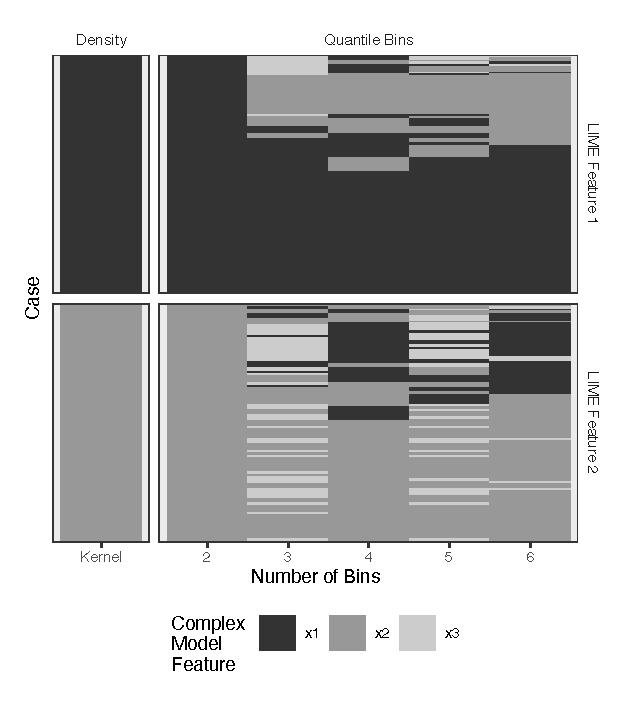
\includegraphics[width=3.125in]{figure-06-1}
%DIFDELCMD <

%DIFDELCMD < }
%DIFDELCMD <

%DIFDELCMD < \end{knitrout}
%DIFDELCMD < %%%
%DIFDELCMD < \caption{%
{%DIFAUXCMD
\emph{\DIFdelFL{Feature Heatmap}}%DIFAUXCMD
\DIFdelFL{. An example feature heatmap of the explanations from the applications of LIME with different tuning parameter values to the \data \ test set. The cases from the test set are plotted on the y-axis, and the tuning parameter values (simulation methods here) are included on the x-axis. The colors of the tiles indicate the feature selected by LIME for the corresponding case and tuning parameter value. The plot is faceted by the first and second most important features selected by LIME (top and bottom facets, respectively). The vertical facets separate the  kernel density method from the quantile bin methods. The vertical striping indicates that the LIME explanations are not consistent across tuning parameter values.}}
%DIFAUXCMD
%DIFDELCMD < \label{fig:figure-06}
%DIFDELCMD < \end{figure}
%DIFDELCMD <

%DIFDELCMD < %%%
\DIFdelend Explanations produced by LIME are likely to be affected by the choice of tuning parameter values. A hypothetical example of this is shown by \DIFdelbegin \DIFdel{Figures \ref{fig:figure-01} and \ref{fig:figure-02} }\DIFdelend \DIFaddbegin \DIFadd{Figure \ref{fig:figure-01} }\DIFaddend where the method used to weight the observations influenced the explanation. As of the time of writing this manuscript, we have encountered no recommendations for how to specify the parameter values besides for the default settings in \DIFaddbegin \DIFadd{the }\DIFaddend \emph{lime} \DIFaddbegin \DIFadd{R package}\DIFaddend . In order to compare the explanations produced by LIME using different tuning parameter values and provide another perspective for assessing localness, we visualize an overview of the explanations with the \emph{feature heatmap} diagnostic plot.

The feature heatmap uses colors to identify the features selected by LIME across multiple predictions (referred to as cases here) and tuning parameter values organized by the feature importance assigned by LIME. That is, for LIME applied with $t$ sets of tuning parameter values to $n$ cases to select the $f$ top features, create $f$ heatmaps (one for each of the positions of importance determined by the magnitude of the explainer model coefficients) with the cases on the $y$-axis, the tuning parameter values on the $x$-axis, and the cells colored by the feature chosen for the corresponding case and tuning parameter value. Additional tuning parameters may also be included in the plot via facets.

\DIFdelbegin \DIFdel{Two hypothetical examples of feature heatmapsare included in }%DIFDELCMD < \autoref{fig:figure-05}%%%
\DIFdel{. The plots are created with the assumption that LIME is applied to select the top feature out of $p=4$  features for $n=10$ cases with $t=5$ sets of tuning parameter values. Situation 1 is  an example where the features selected are consistent across tuning parameter values within a case but vary across cases within a tuning parameter value. This is }\DIFdelend \DIFaddbegin \DIFadd{When interpreting feature heatmaps, horizontal lines of }\DIFaddend the \DIFaddbegin \DIFadd{same color represent the }\DIFaddend ideal situation \DIFdelbegin \DIFdel{, because the LIME explanations }\DIFdelend \DIFaddbegin \DIFadd{where the explanations are consistent and }\DIFaddend do not depend on the tuning \DIFdelbegin \DIFdel{parameters }\DIFdelend \DIFaddbegin \DIFadd{parameter values }\DIFaddend but do depend on the location of the observation in the feature space. \DIFdelbegin \DIFdel{Situation 2 is an example where the selected features vary across tuning parameter values within a case but are consistent across cases within a tuning parameter value. This situation indicates that the features selected by LIME }\DIFdelend \DIFaddbegin \DIFadd{Vertical lines of color represent explanations that }\DIFaddend are dependent on the tuning \DIFdelbegin \DIFdel{parameters, and the explanations }\DIFdelend \DIFaddbegin \DIFadd{parameter values and }\DIFaddend may not be local \DIFdelbegin \DIFdel{, because }\DIFdelend \DIFaddbegin \DIFadd{since }\DIFaddend the same feature is chosen regardless of the \DIFdelbegin \DIFdel{case. In practice, it is expected that the plot will exhibit a combination of these two situations}\DIFdelend \DIFaddbegin \DIFadd{location of the observation in the feature space. See the supporting information for hypothetical examples depicting the extreme cases of feature heatmaps}\DIFaddend .

\DIFdelbegin %DIFDELCMD < \autoref{fig:figure-06} %%%
\DIFdelend \DIFaddbegin \begin{figure}[!tp]
\begin{knitrout}
\definecolor{shadecolor}{rgb}{0.969, 0.969, 0.969}\color{fgcolor}

{\centering \includegraphics[width=3.125in]{figure/figure-04-1}

}



\end{knitrout}
\caption{\emph{\DIFaddFL{Feature Heatmap}}\DIFaddFL{. An example feature heatmap  from applying LIME to the \data \ test set using different tuning parameter values. The vertical striping indicates that the LIME explanations are not consistent across tuning parameter values.}}
\label{fig:figure-04}
\end{figure}

\autoref{fig:figure-04} \DIFaddend shows a feature heatmap for the LIME applications to the 100 observations in the \data \ test set. The most important and second most important features selected by \DIFdelbegin \DIFdel{lime }\DIFdelend \DIFaddbegin \DIFadd{LIME }\DIFaddend are shown in in the top and bottom facets, respectively. For the quantile bins, the original features prior to \DIFdelbegin \DIFdel{the indicator variable transformation }\DIFdelend \DIFaddbegin \DIFadd{being converted to indicator variables }\DIFaddend are included since it is obvious that different features would be selected when the sizes of the bins change. This figure shows that for kernel density and 2-quantile-bins, LIME \DIFdelbegin \DIFdel{selects }\DIFdelend \DIFaddbegin \DIFadd{produces global explanations since }\DIFaddend $x_1$ \DIFaddbegin \DIFadd{is selected }\DIFaddend as the most important feature and $x_2$ \DIFaddbegin \DIFadd{is selected }\DIFaddend as the second most important feature across all cases in the test set. \DIFdelbegin \DIFdel{These explanations are not local. }\DIFdelend There is variability in the features selected by LIME for 3- to \DIFdelbegin \DIFdel{6-quantile-bins }\DIFdelend \DIFaddbegin \DIFadd{6- quantile-bins }\DIFaddend suggesting more local explanations. There are signs of vertical striping, which suggests a dependence on tuning parameters. Note that the explanations from 3- and 5-quantile-bins include the selection of the random noise variable ($x_3$) as an important variable in many predictions\DIFdelbegin \DIFdel{, which should not be the case. The pattern seen in the explanations for 3- to 6-quantile-bins may suggest local explanations, but the dependence on tuning parameters makes it unclear which set of explanations to use}\DIFdelend \DIFaddbegin \sout{, which would not be expected to be important to a random forest}\DIFadd{. It is unclear whether the random forest is using a variable that would not be expected to be important or LIME is incorrectly identifying the important variable when 3- and 5- quantile bins are used}\DIFaddend .

\subsection{Assessment Metric Plot} \label{assess-metric}

\DIFdelbegin %DIFDELCMD < \begin{figure}[!thp]
%DIFDELCMD < \begin{knitrout}
%DIFDELCMD < \definecolor{shadecolor}{rgb}{0.969, 0.969, 0.969}\color{fgcolor}
%DIFDELCMD <

%DIFDELCMD < {\centering \includegraphics[width=3.25in]{figure-07-1}
%DIFDELCMD <

%DIFDELCMD < }
%DIFDELCMD <

%DIFDELCMD < \end{knitrout}
%DIFDELCMD < %%%
%DIFDELCMD < \caption{%
{%DIFAUXCMD
\emph{\DIFdelFL{Assessment metric plot}}%DIFAUXCMD
\DIFdelFL{. The assessment metrics computed on the applications of LIME to the \data \ test set are included in this example assessment metric plot. Each horizontal facet corresponds to one of three metrics: average $R^2$, average fidelity, or MSEE. The LIME tuning parameter values (simulation methods in this example) are plotted on the x-axis, and the metric values are shown on the y-axis. The points are colored by rank (within a metric) indicating best to worst (dark to light). The kernel density simulation methods performs well across all three metrics.}}
%DIFAUXCMD
%DIFDELCMD < \label{fig:figure-07}
%DIFDELCMD < \end{figure}
%DIFDELCMD <

%DIFDELCMD < %%%
\DIFdelend The feature heatmap for the \data \ in the previous section shows an example of inconsistent LIME explanations across tuning parameter values. In this situation, the user must determine which set of explanations to trust. One way to do this is to compute assessment metrics for each set of explanations to identify the optimal tuning parameter values. We discuss three metrics for this purpose and present a visual comparison in an \emph{assessment metric plot}.

Each metric presented below is computed on LIME explanations for a set of predictions obtained using the same tuning parameter values. Here we provide a high level description of the metrics. Notation and formulas for these metrics are included in Appendix \ref{metric-details}.

\begin{itemize}
\item \emph{Average $R^2$}: \DIFdelbegin \DIFdel{Assess }\DIFdelend \DIFaddbegin \DIFadd{Assesses }\DIFaddend the model fit and linearity claim by computing the average of the explainer model $R^2$ values (deviance ratios from the R package \emph{glmnet}).

\item \emph{Average Fidelity}: Measures the faithfulness of the explainer model to the complex model by comparing their predictions. Computed as the average of the explainer model fidelity metrics: a metric presented in \citet{ribeiro:2016} (the weighted distance between explainer and complex model predictions for all observations in the LIME simulated data associated with an individual prediction of interest).

\item \emph{Mean Squared Explanation Error (MSEE)}: Also measures the faithfulness of the explainer model to the complex model by comparing their predictions, but only the prediction of interest is used to compute an average squared deviation between explainer and complex model predictions.
\end{itemize}

\DIFdelbegin %DIFDELCMD < \autoref{fig:figure-07} %%%
\DIFdelend \DIFaddbegin \begin{figure}[!bp]
\begin{knitrout}
\definecolor{shadecolor}{rgb}{0.969, 0.969, 0.969}\color{fgcolor}

{\centering \includegraphics[width=3.25in]{figure/figure-05-1}

}



\end{knitrout}
\caption{\emph{\DIFaddFL{Assessment metric plot}}\DIFaddFL{. This example assessment metric plot  compares different applications of LIME to the \data \ test set. The kernel density simulation method performs well across all three metrics.}}
\label{fig:figure-05}
\end{figure}

\autoref{fig:figure-05} \DIFaddend shows an example assessment metric plot. The three metrics are computed for each of the LIME applications to the \data \ test set. The simulation methods are listed on the x-axis. The plot is faceted by metric, and the metric values are plotted on the y-axis. The \DIFdelbegin \DIFdel{colors of the points }\DIFdelend \DIFaddbegin \DIFadd{point color }\DIFaddend represent the rank of the simulation methods performance based on a particular metric (darker indicates a better metric value and lighter indicates a worse metric value). Higher average $R^2$ values are better, and lower average fidelity and MSEE values are better. This example only includes one tuning parameter: the simulation method. If more than one tuning parameter is considered, the assessment metric plot is extended by adding additional facets\DIFaddbegin \DIFadd{, point shapes, }\DIFaddend or levels to the x-axis.

All three metrics suggest that the kernel density method \DIFdelbegin \DIFdel{performed }\DIFdelend \DIFaddbegin \DIFadd{perform}\sout{ed} \DIFaddend well, but the metrics disagree for the quantile \DIFdelbegin \DIFdel{bins }\DIFdelend \DIFaddbegin \DIFadd{bin}\sout{s} \DIFaddend methods. Average $R^2$ and average fidelity rank the performance of the number of quantile bins the same (2-quantile-bins perform the best and 6-quantile-bins perform the worst). In fact, these two metrics appear to have a mirrored relationship in this example. MSEE provides almost the exact opposite results with 6-quantile-bins performing the best and 2-quantile-bins performing the worst. Average fidelity and MSEE are similar metrics, \DIFdelbegin \DIFdel{so it is not surprising that they would agree in this example. Another factor might be that }\DIFdelend \DIFaddbegin \DIFadd{but }\DIFaddend MSEE only takes the prediction of interest into account and not the full simulated dataset \DIFaddbegin \DIFadd{as average fidelity does. This suggests that 6-quantile-bins produce an explainer model more faithful for the prediction of interest while 2-quantile-bins produce an explainer model more faithful over all simulated data observations (weighted by proximity to the prediction of interest)}\DIFaddend .
\DIFdelbegin \DIFdel{The contradiction between metrics makes it difficult to identify which simulation method to trust.
}\DIFdelend

Recall\DIFdelbegin \DIFdel{that }%DIFDELCMD < \autoref{fig:figure-06} %%%
\DIFdel{indicated that }\DIFdelend \DIFaddbegin \DIFadd{, }\autoref{fig:figure-04} \DIFadd{shows }\DIFaddend the kernel density method \DIFdelbegin \DIFdel{selected the same feature }\DIFdelend \DIFaddbegin \DIFadd{returns the same explanations }\DIFaddend across all cases in the test set \DIFdelbegin \DIFdel{for both the first and second features. It appears that }\DIFdelend \DIFaddbegin \DIFadd{suggesting }\DIFaddend a global trend may be the best explanation for this example\DIFdelbegin \DIFdel{, which }\DIFdelend \DIFaddbegin \DIFadd{. This }\DIFaddend may be reasonable considering that we \DIFdelbegin \DIFdel{know that both }\DIFdelend \DIFaddbegin \DIFadd{would expect }\DIFaddend $x_1$ and $x_2$ \DIFdelbegin \DIFdel{are }\DIFdelend \DIFaddbegin \DIFadd{to be  }\DIFaddend the two features \DIFdelbegin \DIFdel{that should be the features }\DIFdelend used by the random forest to distinguish between response categories. \DIFaddbegin \DIFadd{However, further exploration of individual explanations using explanation scatterplots may help to identify the tuning parameter values that produce the most trustworthy explanations.
}\DIFaddend

\section{Application to Bullet Matching Data} \label{application}

In this section, we \DIFdelbegin \DIFdel{provide a discussion of the application of the }\DIFdelend \DIFaddbegin \DIFadd{apply the }\DIFaddend visual diagnostics for LIME explanations to a practical data problem investigating the similarity of marks on fired bullets.

\subsection{Bullet Matching Data}







In current practice, forensic firearm examiners evaluate whether two bullets are from the same source (fired from the same gun) or from different sources based on microscopic comparison of the striation patterns engraved on bullets during the firing process (see \DIFdelbegin %DIFDELCMD < \autoref{fig:figure-08}%%%
\DIFdelend \DIFaddbegin \autoref{fig:figure-06}\DIFaddend ). The process is based on a visual and therefore subjective assessment of the evidence. The lack of objective evaluation and the associated absence of established error rates has first been criticized by the National Research Council \cite{nrc:2009} and later by the President's Council of Advisors on Science and Technology \cite{pcast:2016}.

In response, \citet{hare:2017} proposed an automated machine learning method for bullet matching to complement a visual inspection by firearm examiners. Based on high-resolution topological scans of land engraved areas, \citet{hare:2017} obtain signatures of striations from two bullet lands (\DIFdelbegin %DIFDELCMD < \autoref{fig:figure-09}%%%
\DIFdelend \DIFaddbegin \autoref{fig:figure-07}\DIFaddend ). Nine features quantifying the similarity of signatures, such as the cross-correlation function, the distance between signatures, and the number of matching striae, are extracted and used to train a random forest to determine the probability of a comparison resulting from the same source (matching signatures) or from different sources (non-matching signatures). The model in \citet{hare:2017} was trained on a set of scans of bullets from the James Hamby Consecutively Rifled Ruger Barrel Study \citep{hamby:2009}, which included 10,384 land-to-land comparisons \DIFdelbegin \DIFdel{\mbox{%DIFAUXCMD
\citet{hare:2017}}\hspace{0pt}%DIFAUXCMD
}\DIFdelend \DIFaddbegin \DIFadd{\mbox{%DIFAUXCMD
\citep{hare:2017}}\hspace{0pt}%DIFAUXCMD
}\DIFaddend . See the supporting information for additional information on the signature similarity features.

\begin{figure}[!t]
\centering
\begin{knitrout}
\definecolor{shadecolor}{rgb}{0.969, 0.969, 0.969}\color{fgcolor}

{\centering \DIFdelbeginFL %DIFDELCMD < 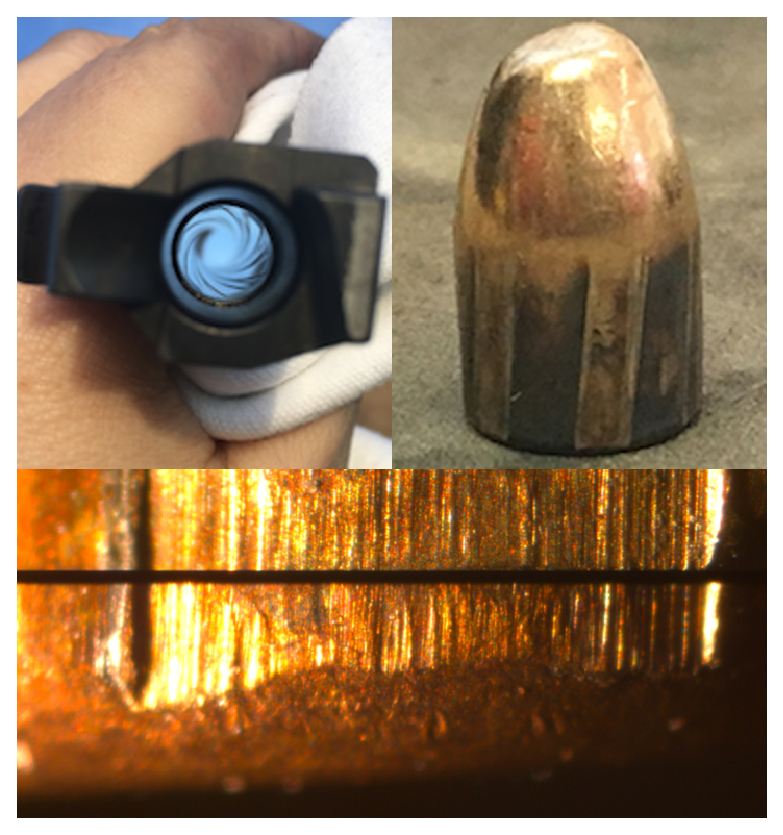
\includegraphics[width=2.25in]{figure-08-1}
%DIFDELCMD < %%%
\DIFdelendFL \DIFaddbeginFL 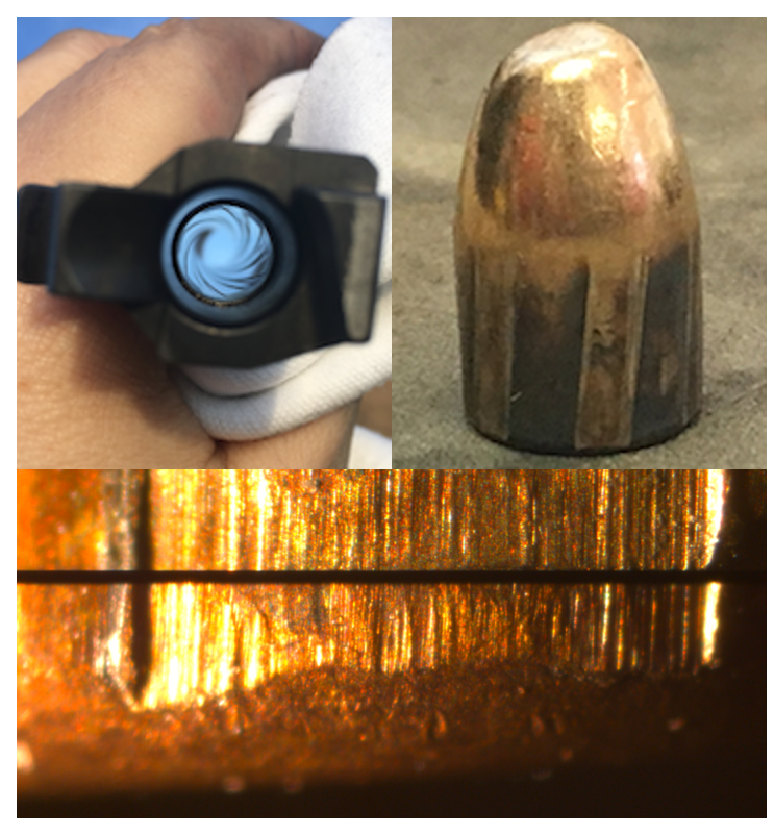
\includegraphics[width=2.25in]{figure-static/figure-06-1}
\DIFaddendFL

}



\end{knitrout}
\caption{(Top left) Traditionally rifled gun barrel. The grooves and lands alternate to give bullets a spin during the firing process, which create markings (striations) on a bullet when fired. (Top right) Image of a fired bullet. The vertical stripes along the lower half of the bullet show groove and land engraved areas. The land engraved areas contain the microscopic striations created when the bullet passed through the barrel of the gun. (Bottom) Close up of a land engraved area showing striations (vertical lines).}
\DIFdelbeginFL %DIFDELCMD < \label{fig:figure-08}
%DIFDELCMD < %%%
\DIFdelendFL \DIFaddbeginFL \label{fig:figure-06}
\DIFaddendFL

\vspace*{\floatsep}

\begin{knitrout}
\definecolor{shadecolor}{rgb}{0.969, 0.969, 0.969}\color{fgcolor}

{\centering \DIFdelbeginFL %DIFDELCMD < \includegraphics[width=3.125in]{figure-09-1}
%DIFDELCMD < %%%
\DIFdelendFL \DIFaddbeginFL \includegraphics[width=3.125in]{figure/figure-07-1}
\DIFaddendFL

}



\end{knitrout}
\caption{Example bullet signatures. The \DIFdelbeginFL \DIFdelFL{bullet }\DIFdelendFL signatures \DIFdelbeginFL \DIFdelFL{correspond to }\DIFdelendFL \DIFaddbeginFL \DIFaddFL{are from }\DIFaddendFL the same land and therefore have very similar patterns.\DIFdelbeginFL \DIFdelFL{The \mbox{%DIFAUXCMD
\citet{hare:2017} }\hspace{0pt}%DIFAUXCMD
random forest is fit using various features that measure the similarity between two such signatures.}\DIFdelendFL }
\DIFdelbeginFL %DIFDELCMD < \label{fig:figure-09}
%DIFDELCMD < %%%
\DIFdelendFL \DIFaddbeginFL \label{fig:figure-07}
\DIFaddendFL \end{figure}

\subsection{Application of LIME to Bullet Matching Data}

\begin{figure*}[!thp]
\begin{knitrout}
\definecolor{shadecolor}{rgb}{0.969, 0.969, 0.969}\color{fgcolor}

{\centering \DIFdelbeginFL %DIFDELCMD < \includegraphics[width=6.5in]{figure-10-1}
%DIFDELCMD < %%%
\DIFdelendFL \DIFaddbeginFL 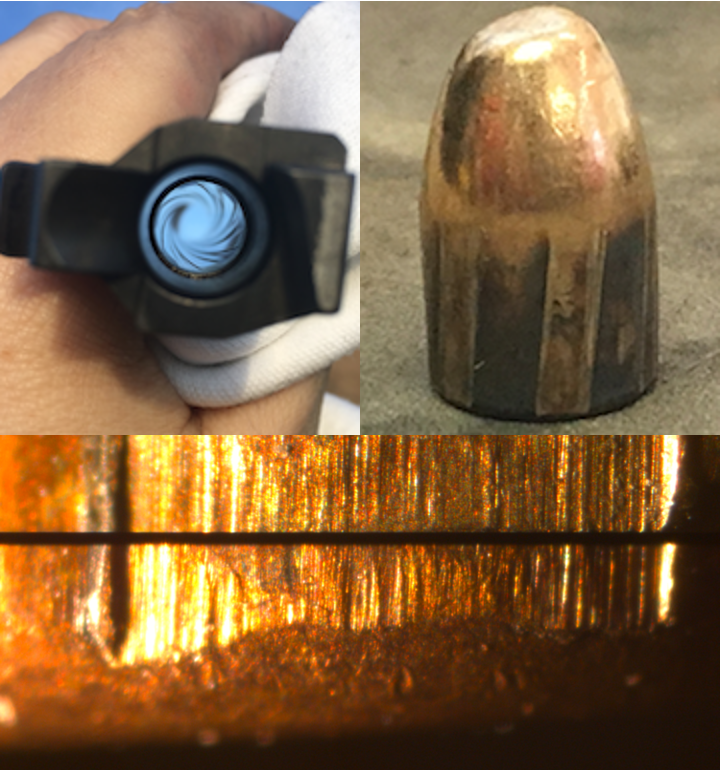
\includegraphics[width=6.5in]{figure-static/figure-08-1}
\DIFaddendFL

}



\end{knitrout}
\caption{Parallel coordinate plots of the \DIFdelbeginFL \DIFdelFL{\mbox{%DIFAUXCMD
\citet{hare:2017} }\hspace{0pt}%DIFAUXCMD
}\DIFdelendFL \DIFaddbeginFL \DIFaddFL{bullet matching }\DIFaddendFL random forest predictions\DIFdelbeginFL \DIFdelFL{from the training (top facet) and testing (bottom facet) data}\DIFdelendFL . \DIFdelbeginFL \DIFdelFL{The observations are separated by known matching (right column) and non-matching (left column) signatures. The y-axis shows the standardized feature values, and the x-axis shows the features used to fit the random forest (ordered by random forest impurity based feature importance). }\DIFdelendFL Each line corresponds to an observation, and the line color represents the associated random forest probability. There are clear relationships between the feature values and the random forest probabilities.}
\DIFdelbeginFL %DIFDELCMD < \label{fig:figure-10}
%DIFDELCMD < %%%
\DIFdelendFL \DIFaddbeginFL \label{fig:figure-08}
\DIFaddendFL \end{figure*}

Since firearm identification is commonly used as evidence for convictions in court cases, it is important to be able to understand and assess a model used to quantify the probability that a bullet is fired from a gun. LIME explanations would provide a local explanation for an individual prediction, but just as it is important to assess the model for this high-stakes application, it is also important to assess the LIME explanations. We will demonstrate an assessment of LIME explanations using the visual diagnostics introduced in this paper.

A random forest model fit to an expanded dataset of 83,028 land-to-land comparisons from two sets of bullets in the James Hamby Consecutively Rifled Ruger Barrel Study \citep{hamby:2009} was validated in \citet{vanderplas:2020}. Here, we train a random forest model to mimic the model validated in \citet{vanderplas:2020} using the same data, model structure, and features (the nine similarity measures developed in \citet{hare:2017}). We apply the trained random forest model to 6 bullets from another set of the Hamby study with 364 rows of land comparisons. See the supporting information for further descriptions of the data.

The newly trained random forest has an out-of-bag accuracy of 1 and out-of-bag false positive and false negative rates of 0.3 and \ensuremath{2\times 10^{-4}}, respectively. On the test data, the random forest performance decreases with an accuracy of 0.85 and false positive and false negative rates of 0.55 and 0.011, respectively. This is an example where explanations of the model predictions could provide insight to the cause of the decrease in model performance on the test data.

\DIFdelbegin \DIFdel{We }\DIFdelend \DIFaddbegin \DIFadd{In }\autoref{fig:figure-08}\DIFadd{, we }\DIFaddend consider a global visualization of the relationship between the random forest predictions and the model features with a parallel coordinate plot of the training data (top \DIFdelbegin \DIFdel{facet}\DIFdelend \DIFaddbegin \DIFadd{row}\DIFaddend ) and testing data (bottom \DIFdelbegin \DIFdel{facets)(}%DIFDELCMD < \autoref{fig:figure-10}%%%
\DIFdel{)}\DIFdelend \DIFaddbegin \DIFadd{row)}\DIFaddend . In the training data we observe a clear difference in feature values based on whether the corresponding random forest scores are close to 1 or 0. High values of rough correlation, cross correlation function, and number of matches are indicative of random forest scores close to 1; similarly, low values of mismatches, distance, and non-consecutively matching striae are also associated with random forest scores close to 1. Observations in the test data that are classified incorrectly by the random forest tend to have feature values similar to observations in the training data with similar random forest scores.
\DIFdelbegin \DIFdel{For example, the observations in the test set known to be a match but have a random forest score below 0.5 have relatively low values of rough correlation, cross correlation function, and matches and relatively large values of mismatches, distance, and non-consecutively matching striae compared to observations with a random forest probability close to 1.
}\DIFdelend

LIME is applied to all test set observations using different tuning parameter values: 12 sampling methods (\DIFdelbegin \DIFdel{2 to 6 equally spaced bins, 2 to 6 }\DIFdelend \DIFaddbegin \DIFadd{2- to 6- equally-spaced bins, 2- to 6- }\DIFaddend quantile-bins, kernel density estimation, and normal approximation) and 3 Gower exponents (0.5, 1, and 10). Thus, a total of $12\times 3=36$ different applications of LIME are performed. We specify that each LIME explanation return 3 features, and feature selection is performed using the default option in LIME, which selects the features with the highest weights in a ridge regression model.







\subsection{LIME Assessment Visualizations} \label{bullet-assess-ex}

To get an overview of the LIME explanations from the 36 applications, we consider a feature heatmap (\DIFdelbegin %DIFDELCMD < \autoref{fig:figure-11}%%%
\DIFdelend \DIFaddbegin \autoref{fig:figure-09}\DIFaddend ). In addition to facets for simulation method and LIME feature importance, this plot includes a vertical facet for Gower power and a horizontal facet for whether the observation is a known match or non-match. This plot highlights several key features of the LIME explanations from the bullet matching dataset.

First, applications of \DIFdelbegin \DIFdel{2-quantile-bin }\DIFdelend \DIFaddbegin \DIFadd{2-quantile-bins, 2-equal-bins, and somewhat for the density based }\DIFaddend simulations produce the same explanations for almost all cases and LIME tuning parameter values\DIFdelbegin \DIFdel{. This suggests that the LIME }\DIFdelend \DIFaddbegin \DIFadd{, suggesting these }\DIFaddend explanations are global and not local. Second, within a simulation method, the features selected by LIME for an observation do not appear to vary by the Gower power. However, the LIME \DIFdelbegin \DIFdel{explanation }\DIFdelend \DIFaddbegin \DIFadd{explanations }\DIFaddend for an observation often \DIFdelbegin \DIFdel{varies }\DIFdelend \DIFaddbegin \DIFadd{vary }\DIFaddend across simulation methods. With the \DIFdelbegin \DIFdel{equal-bins}\DIFdelend \DIFaddbegin \DIFadd{equal bins}\DIFaddend , there are vertical stripes that suggest a dependence of the LIME explanations on the number of bins. The vertical stripes are not as apparent with the quantile bins. Lastly, there are clear differences between the LIME explanations produced by the bin based simulation methods for the matches and non-matches. This suggests that different features are of importance in the random forest, depending on whether the observation corresponds to match or non-match.

\begin{figure*}[!thp]
\begin{knitrout}
\definecolor{shadecolor}{rgb}{0.969, 0.969, 0.969}\color{fgcolor}

{\centering \DIFdelbeginFL %DIFDELCMD < \includegraphics[width=6.5in]{figure-11-1}
%DIFDELCMD < %%%
\DIFdelendFL \DIFaddbeginFL \includegraphics[width=6.5in]{figure/figure-09-1}
\DIFaddendFL

}



\end{knitrout}
\caption{Feature heatmap of 36 LIME applications to the bullet comparison data test set. \DIFdelbeginFL \DIFdelFL{In addition to faceting the results by simulation method and LIME feature selection order, facets for the Gower power and whether the observation is a match or non-match are included. }\DIFdelendFL The vertical stripes of features selected indicate a dependence between the LIME explanations and tuning parameter values.}
\DIFdelbeginFL %DIFDELCMD < \label{fig:figure-11}
%DIFDELCMD < %%%
\DIFdelendFL \DIFaddbeginFL \label{fig:figure-09}
\DIFaddendFL

\vspace*{\floatsep}

\begin{knitrout}
\definecolor{shadecolor}{rgb}{0.969, 0.969, 0.969}\color{fgcolor}

{\centering \DIFdelbeginFL %DIFDELCMD < 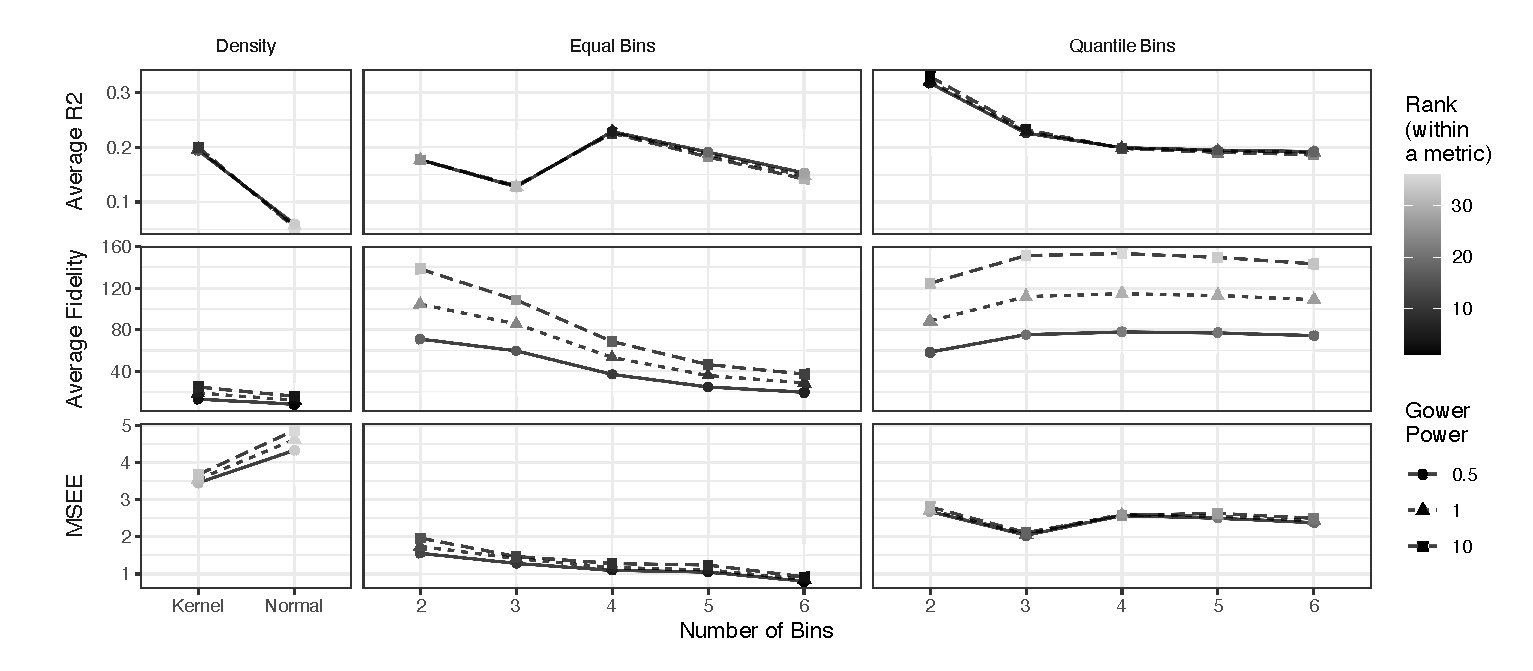
\includegraphics[width=6.5in]{figure-12-1}
%DIFDELCMD < %%%
\DIFdelendFL \DIFaddbeginFL \includegraphics[width=6.5in]{figure/figure-10-1}
\DIFaddendFL

}



\end{knitrout}
\caption{Assessment metric plot \DIFdelbeginFL \DIFdelFL{for the applications of }\DIFdelendFL \DIFaddbeginFL \DIFaddFL{comparing }\DIFaddendFL LIME \DIFdelbeginFL \DIFdelFL{on }\DIFdelendFL \DIFaddbeginFL \DIFaddFL{results from applications to }\DIFaddendFL the bullet comparison data test set. There are discrepancies in \DIFdelbeginFL \DIFdelFL{performance across metrics for a set of tuning parameter values}\DIFdelendFL \DIFaddbeginFL \DIFaddFL{metric performances}\DIFaddendFL , but \DIFdelbeginFL \DIFdelFL{based on the }\DIFdelendFL overall\DIFdelbeginFL \DIFdelFL{performance of all three metrics}\DIFdelendFL , \DIFdelbeginFL \DIFdelFL{4-equal-bins }\DIFdelendFL \DIFaddbeginFL \DIFaddFL{the 4-equal-bin implementation }\DIFaddendFL with a Gower power of 0.5 appears to perform the best.}
\DIFdelbeginFL %DIFDELCMD < \label{fig:figure-12}
%DIFDELCMD < %%%
\DIFdelendFL \DIFaddbeginFL \label{fig:figure-10}
\DIFaddendFL \end{figure*}

To try to identify a set of LIME tuning parameter values with the most trustworthy set of explanations, an assessment metric plot is considered (\DIFdelbegin %DIFDELCMD < \autoref{fig:figure-12}%%%
\DIFdelend \DIFaddbegin \autoref{fig:figure-10}\DIFaddend ). The performance of a set of tuning parameter values often do not agree across metrics. For example, both density methods perform well according to average fidelity but poorly according to MSEE. All quantile bin methods perform well according to average $R^2$ but poorly based on average fidelity and MSEE. However, there is consistency in results across different Gower powers. The applications using a power of 0.5 perform the best or as well as the other powers across all simulation methods suggesting that the power that leads to a more \DIFdelbegin \DIFdel{global }\DIFdelend \DIFaddbegin \DIFadd{local }\DIFaddend explanation is preferred\DIFdelbegin \DIFdel{by LIME}\DIFdelend . It is not \DIFdelbegin \DIFdel{apparent }\DIFdelend \DIFaddbegin \DIFadd{obvious  }\DIFaddend which set of tuning parameters is the best\DIFdelbegin \DIFdel{. Considering }\DIFdelend \DIFaddbegin \DIFadd{, but considering }\DIFaddend all three metrics, we might conclude that the 4-equal-bins with a Gower power of 0.5 performs better than the other tuning parameter values considered.

\DIFdelbegin \DIFdel{To provide }\DIFdelend \DIFaddbegin \DIFadd{For }\DIFaddend a more detailed view of explanations \DIFdelbegin \DIFdel{obtained using }\DIFdelend \DIFaddbegin \DIFadd{based on }\DIFaddend different tuning parameter values, we \DIFdelbegin \DIFdel{take a closer look at explanations for two observations }\DIFdelend \DIFaddbegin \DIFadd{consider explanation scatterplots for a prediction }\DIFaddend of interest, \DIFdelbegin \DIFdel{which will be referred to as case M (a known match) and case NM (a known }\DIFdelend \DIFaddbegin \DIFadd{a known }\DIFaddend non-match \DIFdelbegin \DIFdel{), using explanation scatterplots. Figure~\ref{fig:figure-13} includes the visual representation plots of explanations (from }\DIFdelend \DIFaddbegin \DIFadd{(NM), in Figure~\ref{fig:figure-11} along with the explanation plots from the }\DIFaddend \emph{lime} \DIFdelbegin \DIFdel{) and explanation scatterplots for cases M and NM}\DIFdelend \DIFaddbegin \DIFadd{R package}\DIFaddend . Plots for 4-equal-bins and 4-quantile-bins are included to depict tuning parameter values with good (4-equal-bins) and mediocre (4-quantile-bins) performance based on the assessment metric plot. \DIFdelbegin \DIFdel{Plots for }\DIFdelend \DIFaddbegin \DIFadd{Additional examples of explanation scatterplots including explanations for a known match and explanations produced using }\DIFaddend the kernel density simulation method are included in \DIFdelbegin \DIFdel{Appendix~\ref{exp-scatter_plus} (Figure \ref{fig:figure-B2}) .
}\DIFdelend \DIFaddbegin \DIFadd{the supporting information.
}\DIFaddend

\DIFdelbegin \DIFdel{We focus on the explanation for case NM with }\DIFdelend \DIFaddbegin \DIFadd{Figure~\ref{fig:figure-11} (top left) shows that when }\DIFaddend 4-quantile-bins \DIFdelbegin \DIFdel{. The explanation plot from }\emph{\DIFdel{lime}} %DIFAUXCMD
\DIFdel{shows that the observed values of NM of mismatchesless than or equal to 7.17}\DIFdelend \DIFaddbegin \DIFadd{are applied to case NM, LIME finds the values of mismatches}\DIFaddend , rough correlation\DIFdelbegin \DIFdel{(rough\_cor) greater than 0.05, and D less than or equal to 0.002 support a }\DIFdelend \DIFaddbegin \DIFadd{, and distance are important and support a prediction of the class true. However, this explanation contradicts the }\DIFaddend random forest prediction \DIFdelbegin \DIFdel{in favor of a match. The scatter plots show that many of the simulated values in the rectangular regions with mismatches less than 7.17, rough correlation greater than 0.05, and distance less than or equal to 0.002 have }\DIFdelend \DIFaddbegin \DIFadd{which correctly assigns the observation a non-match. The explanation scatterplot (Figure~\ref{fig:figure-11} bottom left) clarifies the reason. Case NM falls on the boundary of regions for each of these three features where the }\DIFaddend random forest predictions \DIFdelbegin \DIFdel{greater than }\DIFdelend \DIFaddbegin \DIFadd{transition from below }\DIFaddend 0.5 \DIFdelbegin \DIFdel{, which agrees with the LIME explanation}\DIFdelend \DIFaddbegin \DIFadd{to above 0.5}\DIFaddend . However, the \DIFdelbegin \DIFdel{random forest assigns a probability of 0.21 to case NM }\DIFdelend \DIFaddbegin \DIFadd{regions used when applying LIME from the 4-quantile-bins where case NM falls contain mostly observations with random forest predictions above 0.5, leading to the unfaithful explanation.
}

\DIFadd{Figure~\ref{fig:figure-11} (top right) shows that when 4-equal-bins are used, the features LIME identifies as important are distance and mismatches, which support a match and matches, which supports a non-match. This explanation is more faithful having at least one feature supporting a non-match and has a better linear fit, but the most important feature identified by LIME still supports a match, contradicting the random forest. The explanation scatterplot (Figure~\ref{fig:figure-11} bottom right) again shows the features supporting a match arise from NM falling on the boundary of random forest prediction regions that are not well captured by the LIME bins.
}

\DIFadd{Without an assessment of the LIME explanations}\DIFaddend , \DIFdelbegin \DIFdel{which is not explained by the LIME explanationthat provides all explanations in support of a match . Instead, consider that a better explanation based on the scatterplots would be that the random forest assigned a prediction probably below 0.5 since NM has observed values of mismatches less than 5, rough correlation greater than 0.25, and distance greater than 0.001. }%DIFDELCMD <

%DIFDELCMD < %%%
\DIFdel{The other explanation scatterplots can be interpreted in a similar manner. The three plots depict situations where the explanations are faithful to the random forest , but the regions captured by the intersections of the bins do not align well with the regions containing similar probabilities produced by the random forest}\DIFdelend \DIFaddbegin \DIFadd{the default method would produce poor explanations such as the one shown in Figure~\ref{fig:figure-11} (left column). Our assessment here led to better explanations when the four equal bins are used. However, the explanation quality is still lacking from the one prediction considered. Additional investigations using explanations scatterplots would help to determine whether to trust this set of explanations, continue tuning the LIME parameters, or use another approach to provide better insight}\DIFaddend .

\begin{figure*}[!thp]
\begin{knitrout}
\definecolor{shadecolor}{rgb}{0.969, 0.969, 0.969}\color{fgcolor}

{\centering \DIFdelbeginFL %DIFDELCMD < \includegraphics[width=6.25in]{figure-13-1}
%DIFDELCMD < %%%
\DIFdelendFL \DIFaddbeginFL \includegraphics[width=6.25in]{figure/figure-11-1}
\DIFaddendFL

}



\end{knitrout}
\DIFdelbeginFL %DIFDELCMD < \caption{%
{%DIFAUXCMD
\DIFdelFL{Plots of LIME explanations (first and third rows) and explanation scatterplots (second and fourth rows) for  cases M and NM in the bullet test data for two tuning parameter values: 4-quantile-bins (first column) and 4-equal-bins (second column).  The plots provide insights into the LIME explanations and allow for the assessment of the explanation quality.}}
%DIFAUXCMD
%DIFDELCMD < \label{fig:figure-13}
%DIFDELCMD < %%%
\DIFdelendFL \DIFaddbeginFL \caption{\DIFaddFL{Plots of LIME explanations (first row) and explanation scatterplots (second row) for case NM in the bullet test data for two tuning parameter values: 4-quantile-bins (first column) and 4-equal-bins (second column).}}
\label{fig:figure-11}
\DIFaddendFL \end{figure*}
\DIFdelbegin %DIFDELCMD <

%DIFDELCMD < %%%
\DIFdel{Without applying LIME with multiple tuning parameter values to the bullet test data or viewing diagnostic plots of the LIME explanations, it may be very possible to formulate reasons why the LIME explanations make sense. However, the sequence of plots in this section (Figures \ref{fig:figure-11} , \ref{fig:figure-12}, and \ref{fig:figure-13})suggest that we should be cautious to trust any of these LIME explanations . It appears that either LIME needs to be further tuned to provide trustworthy and good explanations, or a different approach may provide better insight.
}\DIFdelend

\section{Discussion} \label{discussion}

This paper highlights that while an explainer model is meant to provide clarity, it actually adds another layer of complexity to predictive models by requiring yet another model that needs to be assessed. Without an assessment of the explainer model, LIME is a black-box procedure \DIFdelbegin \DIFdel{of its own }\DIFdelend requiring blind trust in the explainer model. We suggest the use of visual diagnostics to counteract the black-box nature of LIME\DIFdelbegin \DIFdel{and }\DIFdelend \DIFaddbegin \DIFadd{. We }\DIFaddend provide three diagnostic plots \DIFdelbegin \DIFdel{.
}%DIFDELCMD <

%DIFDELCMD < %%%
\DIFdel{The visualizations are intended to provide insight on how LIME works, assess the ability of the explainer model to capture the complex predictive model, and compare LIME explanations produced by different tuning parameter values. While the visualizations accomplish these tasks, they also expose examples of the failings of LIME. To address the discovered failings of LIME, we }\DIFdelend \DIFaddbegin \DIFadd{intended to assess whether LIME explanations meet the claims made by \mbox{%DIFAUXCMD
\citet{ribeiro:2016}}\hspace{0pt}%DIFAUXCMD
. The examples in this paper bring to light many scenarios in which the claims are not met or are difficult to assess. We }\DIFaddend reconsider each of the claims \DIFdelbegin \DIFdel{about the performance of LIME made by \mbox{%DIFAUXCMD
\citet{ribeiro:2016} }\hspace{0pt}%DIFAUXCMD
in light of the insights gained from the diagnostic visualizations}\DIFdelend \DIFaddbegin \DIFadd{and how the visual diagnostics identify their failings}\DIFaddend .

As previously discussed, the \textbf{interpretability} of the LIME explanations is controllable by the complexity of the explainer model. For example, the number of bins selected for simulation \DIFdelbegin \DIFdel{can control }\DIFdelend \DIFaddbegin \DIFadd{controls }\DIFaddend the interpretability of the explanations. If too many bins are selected, the bin range that is reported in the LIME explanation will be too small to be meaningful in the context of the feature. An appropriate choice of the number of bins will keep the bin range meaningful. Thus, the claim of interpretability does not need to be assessed using the visualizations. However, diagnostic visualizations do present a different perspective on the meaning of interpretability.

Even though an explanation will be interpretable \DIFdelbegin \DIFdel{as long as }\DIFdelend \DIFaddbegin \DIFadd{if  }\DIFaddend the complexity of the explainer model is appropriately chosen, a lack of understanding of the \DIFdelbegin \DIFdel{process used to create the explanation }\DIFdelend \DIFaddbegin \DIFadd{explainer model }\DIFaddend could lead to an incorrect interpretation of the explanation. For example, the visualization of a LIME explanation \DIFdelbegin \DIFdel{available }\DIFdelend from the \emph{lime} R package \citep{pedersen:2020} (\DIFdelbegin \DIFdel{shown in Figures \ref{fig:figure-04} and \ref{fig:figure-13}) is a major }\DIFdelend \DIFaddbegin \autoref{fig:figure-03} \DIFadd{left; }\autoref{fig:figure-11} \DIFadd{top) provides an (over-)}\DIFaddend simplification of the explainer model \DIFdelbegin \DIFdel{, which }\DIFdelend \DIFaddbegin \DIFadd{that }\DIFaddend could lead to \DIFdelbegin \DIFdel{under-interpreted or misinterpreted LIME explanation}\DIFdelend \DIFaddbegin \DIFadd{misinterpreted LIME explanations}\DIFaddend . Supplementing \citet{pedersen:2020}'s compact visualization of the explanation with an explanation scatterplot that shows a more detailed visualization of the explainer model promotes a more complete understanding of the explanation (\DIFdelbegin \DIFdel{such as Figures~\ref{fig:figure-04} and \ref{fig:figure-13}}\DIFdelend \DIFaddbegin \autoref{fig:figure-03} \DIFadd{right; }\autoref{fig:figure-11} \DIFadd{bottom}\DIFaddend ).

Even with an explainer model that is interpreted correctly, the interpretation is worthless if the explainer model is not \textbf{faithful} to the complex model. \DIFdelbegin \DIFdel{This claim can be assessed using the diagnostic plots suggested in this paper. Many of the visualizations in this paper highlight problems with the faithfulness of the explainer models. The explanation }\DIFdelend \DIFaddbegin \DIFadd{Explanation }\DIFaddend scatterplots allow for a comparison of the explainer model to the complex model. The examples in this paper show cases where the explainer model \DIFaddbegin \DIFadd{oversimplifies the model and }\DIFaddend bins do not accurately capture the regions with similar random forest probabilities that contain the prediction of interest \DIFdelbegin \DIFdel{and oversimplify the model (Figures \ref{fig:figure-04} and \ref{fig:figure-13}}\DIFdelend \DIFaddbegin \DIFadd{(}\autoref{fig:figure-03} \DIFadd{right; }\autoref{fig:figure-11} \DIFadd{bottom}\DIFaddend ). Using fewer bins would clearly not help improve the faithfulness of the explainer model in these examples, and while an increase in the number of bins would lead to a finer resolution of the random forest classification boundaries, interpretability of the explainer model would quickly be lost. Perhaps this could be improved by allowing the bin creation to account for the relationships between the features and response variable or a different number of bins for each feature.

\DIFdelbegin \DIFdel{In addition to assessing faithfulness by visually comparing the complex and explainer model, we propose a }\DIFdelend \DIFaddbegin \DIFadd{We also propose an assessment metric plot for the }\DIFaddend visual comparison of two faithfulness metrics\DIFdelbegin \DIFdel{(}\DIFdelend \DIFaddbegin \DIFadd{: }\DIFaddend MSEE and average fidelity\DIFdelbegin \DIFdel{). The examples of faithfulnessmetric comparisons in this paper both produced conflicting results (Figures \ref{fig:figure-07} and \ref{fig:figure-12}). This makes it difficult to decide on a recommendation of a set of tuning parameter values that produce the explanations with the most faithful explainer model}\DIFdelend . \DIFaddbegin \DIFadd{Both metrics measure faithfulness, but MSEE only accounts for the prediction of interest while average fidelity accounts for all observations in the simulated data. As a result, the measures may disagree (Figures \ref{fig:figure-05} and \ref{fig:figure-10}), and the user is left to determine which is preferable.
}\DIFaddend

The metric comparison plot also includes a comparison of average $R^2$ values, which is a metric that can be used to assess the claim of \textbf{linearity}. Most of the average $R^2$ values in the examples from this paper are below 0.5 suggesting a poor linear fit of the explainer models. A poor linear fit of the explainer model is also seen with the residual plot \DIFdelbegin \DIFdel{(}%DIFDELCMD < \autoref{fig:figure-C3}%%%
\DIFdel{)}\DIFdelend \DIFaddbegin \DIFadd{shown in }\autoref{fig:figure-B1}\DIFaddend .

The final claim, \textbf{localness}, is addressed by \DIFdelbegin \DIFdel{the feature heatmap and metric comparison plots. As stated, the feature heatmap reveals that the density simulation methods in the \data \ example  results in global explanations where the same features are repeatedly chosen across all (or almost all ) observations in the set of explanations. This finding agrees with that of \mbox{%DIFAUXCMD
\citet{laugel:2018} }\hspace{0pt}%DIFAUXCMD
who found LIME produced global explanations with the normal approximation simulation method. For the bin based simulation methods in the bullet data example, the feature heatmap shows that the features chosen for the explanations vary between the two classification categories (match versus non-match). This is an interesting finding that suggests that different features can play a role in the predictions of observations in different response categories. Furthermore, while the metric comparison plot in the bullet example does not provide agreement between metrics on a best bin based method, all metrics agree that a Gower power of 0.5 for computing the model weights associated with distance of a simulated data point from the prediction of interest is the best. This suggests that a less local explanation provides a better explanation of the performance of the random forest}\DIFdelend \DIFaddbegin \DIFadd{feature heatmaps and explanation scatterplots. The vertical stripes seen in the feature heatmaps (Figures \ref{fig:figure-04} and \ref{fig:figure-09}) suggest global explanations produced by LIME since the same explanation is returned for almost all observations regardless of feature values. The explanation scatterplots visualize the locality of the explanation using point size to indicate weight. However, the lack of definition of a local region makes it difficult to assess whether the weights capture an appropriately local region}\DIFaddend .

\DIFdelbegin \DIFdel{Some of the visualizations in the paper generalize easily to any application of LIME such as the feature heatmap and metric plot. Other plots such as the }\DIFdelend \DIFaddbegin \DIFadd{These diagnostic visualizations are a starting point that already highlight seemingly common issues with the LIME claims. Additions, such as }\DIFaddend visualizations of the \DIFdelbegin \DIFdel{LIME procedure would require extensions such as the use of scatterplot matrices to compare explanations with more than two features. The addition of interactivity to the diagnostic plots would provide additional enhancement of }\DIFdelend \DIFaddbegin \DIFadd{step-by-step process of the creation of LIME explanations and interactivity would enhance }\DIFaddend the assessment process. For example, a diagnostic plot that provides a summary of multiple LIME explanations, such as the feature heatmap, could be \DIFdelbegin \DIFdel{displayed and }\DIFdelend clicked on to reveal more detailed figures\DIFdelbegin \DIFdel{associated with individual predictions of interest}\DIFdelend , such as an explanation scatterplot\DIFaddbegin \DIFadd{, for a prediction of interest}\DIFaddend .

The largest limitation to the diagnostic visualizations is the dimensionality of the data shown, both in the number of dimensions or features as well as the number of observations. Fortunately, in the situation of LIME, both of these aspects are rather well controlled: LIME relies heavily on simulations to generate data scenarios that are close to the data observed but exhibit variability. Effects from overplotting should be relatively mild, because output from simulations is shown, which is expected to be (relatively) continuous such that overplotting only occurs for points with (relatively) similar values. In that respect, the diagnostics shown for the \data \ and the bullet example are representative of what is expected. But in cases where overplotting does become problematic, the user could either simply reduce the size of the simulations or use some well-studied binning techniques in the visualizations, as discussed for example in \citet{carr:1987} or \citet{unwin:2006}.

While it would be ideal if LIME could be used as a method to provide easily understandable explanations for black-box models as \citet{ribeiro:2016} claim, \DIFdelbegin \DIFdel{that dream is not yet a }\DIFdelend \DIFaddbegin \DIFadd{there is still work to be done to achieve that }\DIFaddend reality. The examples using diagnostic plots to assess LIME in this paper show frequent \DIFdelbegin \DIFdel{issues with LIME }\DIFdelend \DIFaddbegin \DIFadd{instances when the claims about LIME are not met}\DIFaddend . We hope that our plots provide motivation to assess LIME explanations, to not blindly use the default settings (even if \DIFdelbegin \DIFdel{it is not clear }\DIFdelend how to tune the parameters \DIFaddbegin \DIFadd{is not clear}\DIFaddend ), and to encourage work \DIFdelbegin \DIFdel{on }\DIFdelend improving LIME, so that it can be a lime and not a lemon.

\section*{Acknowledgments}

HH was partially funded by the Center for Statistics and Applications in Forensic Evidence (CSAFE) through Cooperative Agreement 70NANB20H019 between NIST and Iowa State University, which includes activities carried out at Carnegie Mellon University, Duke University, University of California Irvine, University of Virginia, West Virginia University, University of Pennsylvania, Swarthmore College and University of Nebraska, Lincoln.

\subsection*{Author contributions}

{\bf Katherine Goode, Heike Hofmann}: Conceptualization, Methodology, Investigation, Visualizations, Writing - Reviewing and Editing. {\bf Katherine Goode}: Writing - Initial Draft, Software.

\subsection*{Financial disclosure}

None reported.

\subsection*{Conflict of interest}

The authors declare no potential conflict of interests.

\section*{Supporting information}

\DIFdelbegin \DIFdel{The code used to produce the manuscript and the data from examples in Section \ref{application} are available in the }\DIFdelend \DIFaddbegin \DIFadd{Additional examples of the visual diagnostics and more info on the bullet matching data may be found in the Supporting Information section of the online version of the manuscript. The code  and  data associated with the manuscript are also included in the online Supporting Information section and  in the }\DIFaddend following GitHub Repository: \href{https://github.com/goodekat/LIME-diagnostics-paper}{https://github.com/goodekat/LIME-diagnostics-paper}.

\bibliography{references}

\newpage

\appendix

\section{LIME Tuning Parameter Options} \label{lime-details}

The following tuning parameters for the LIME algorithm are available in the \emph{lime} R package \citep{pedersen:2020}.

\begin{itemize}

\item Data simulation methods:

\begin{itemize}
\item Equally spaced bins: observations are uniformly sampled from equally spaced bins (number of bins may be specified)
\item Quantile bins: observations are uniformly sampled from quantile bins (number of bins may be specified)
\item Normal density approximation: observations are sampled from a normal distribution with mean and standard deviation computed from the corresponding feature
\item Kernel density approximation: observations are sampled from an kernel density approximation of the corresponding feature
\end{itemize}

\item Number of observations to simulate

\item Distance metric for determining proximity to the prediction of interest: Gower distance (where the power may be specified) or exponential kernel (where the kernel width may be specified)

\item Number of features to return in an explanation

\item Feature selection method for determining the features to return in an explanation: forward selection applied to a ridge regression, features with the largest magnitude coefficients in ridge regression, LASSO, classification/regression tree splits

\end{itemize}

\DIFdelbegin \section{\DIFdel{Explanation Scatterplots Under Other Simulation Scenarios}} %DIFAUXCMD
\addtocounter{section}{-1}%DIFAUXCMD
%DIFDELCMD < \label{exp-scatter_plus}
%DIFDELCMD <

%DIFDELCMD < %%%
\DIFdel{Section \ref{exp-scatter} introduces explanation scatterplots under the default simulation method in the }\DIFdelend \DIFaddbegin \DIFadd{The }\DIFaddend \emph{lime} R package \DIFdelbegin \DIFdel{: 4-quantile-bins. The structure of an explanation scatterplot remains the same if any bin based simulation method is used, i.e., any number of quantile or equally spaced bins. However, if the kernel density or normal approximation simulation methods are used, the format of the explanation scatterplot changes. In the density based simulation method scenarios, LIME uses the standardized versions of the predictor variables to fit the }\DIFdelend \DIFaddbegin \DIFadd{uses a ridge regression fit using the }\emph{\DIFadd{glmnet}} \DIFadd{R package \mbox{%DIFAUXCMD
\citep{simon:2011} }\hspace{0pt}%DIFAUXCMD
as the }\DIFaddend explainer model. \DIFdelbegin \DIFdel{Thus, the explainer model needs to be represented differently in the explanation scatterplot.
}\DIFdelend \DIFaddbegin \DIFadd{Note that the ridge regression penalty parameter (referred to as $\lambda$ in }\emph{\DIFadd{glmnet}}\DIFadd{) is usually treated as a tuning parameter, but the }\emph{\DIFadd{lime}} \DIFadd{R package always sets $\lambda$ to 2 divided by the number of observations in the simulated dataset.
}\DIFaddend

\DIFdelbegin \DIFdel{When the kernel density or normal approximation simulation methods are applied, the explanation scatterplot depicts the complex model by plotting the complex model predictions versus a feature selected in LIME the explanation from the simulated data. The explainer model is included as a line on the figure where all features excluding the one plotted on the x-axis are set to the observed values of the prediction of interest. An explanation scatterplot is created for each feature included in the LIME explanation.
As with the bin based simulation method, the size of the points represent the weight assigned by LIME.
}%DIFDELCMD <

%DIFDELCMD < %%%
\DIFdel{Figure \ref{fig:figure-B1} provides example explanation scatterplots for each feature in the default LIME explanation obtained using the kernel density simulation method for the \data \ prediction of interest. Figure \ref{fig:figure-B2} includes explanation scatterplots for the explanations generated using kernel density simulation for the bullet example cases M and NM discussed in Section \ref{bullet-assess-ex}.
}%DIFDELCMD <

%DIFDELCMD < \begin{figure*}[!thp]
%DIFDELCMD < %%%
\DIFdelendFL \DIFaddbeginFL \section{\DIFaddFL{Explainer Model Residual Plot}} \label{residual-plot}
\begin{figure}[!h]
\DIFaddendFL \begin{knitrout}
\definecolor{shadecolor}{rgb}{0.969, 0.969, 0.969}\color{fgcolor}

{\centering \DIFdelbeginFL %DIFDELCMD < \includegraphics[width=6.5in]{figure-B1-1}
%DIFDELCMD < %%%
\DIFdelendFL \DIFaddbeginFL \includegraphics[width=3.125in]{figure/figure-B1-1}
\DIFaddendFL

}



\end{knitrout}
\caption{\DIFdelbeginFL \DIFdelFL{Explanation scatterplots for }\DIFdelendFL \DIFaddbeginFL \DIFaddFL{Residual plot of }\DIFaddendFL the \DIFaddbeginFL \DIFaddFL{explainer model associated with }\DIFaddendFL \data \ prediction of interest \DIFdelbeginFL \DIFdelFL{with }\DIFdelendFL \DIFaddbeginFL \DIFaddFL{from Section \ref{exp-scatter}, which suggests a violation of }\DIFaddendFL the \DIFdelbeginFL \DIFdelFL{kernel density simulation method}\DIFdelendFL \DIFaddbeginFL \DIFaddFL{linearity assumption}\DIFaddendFL .}
\label{fig:figure-B1}
\DIFdelbeginFL %DIFDELCMD < \end{figure*}
%DIFDELCMD < %%%
\DIFdelend \DIFaddbegin \end{figure}
\DIFaddend

\DIFdelbegin %DIFDELCMD < \begin{figure*}[!thp]
%DIFDELCMD < \begin{knitrout}
%DIFDELCMD < \definecolor{shadecolor}{rgb}{0.969, 0.969, 0.969}\color{fgcolor}
%DIFDELCMD <

%DIFDELCMD < {\centering 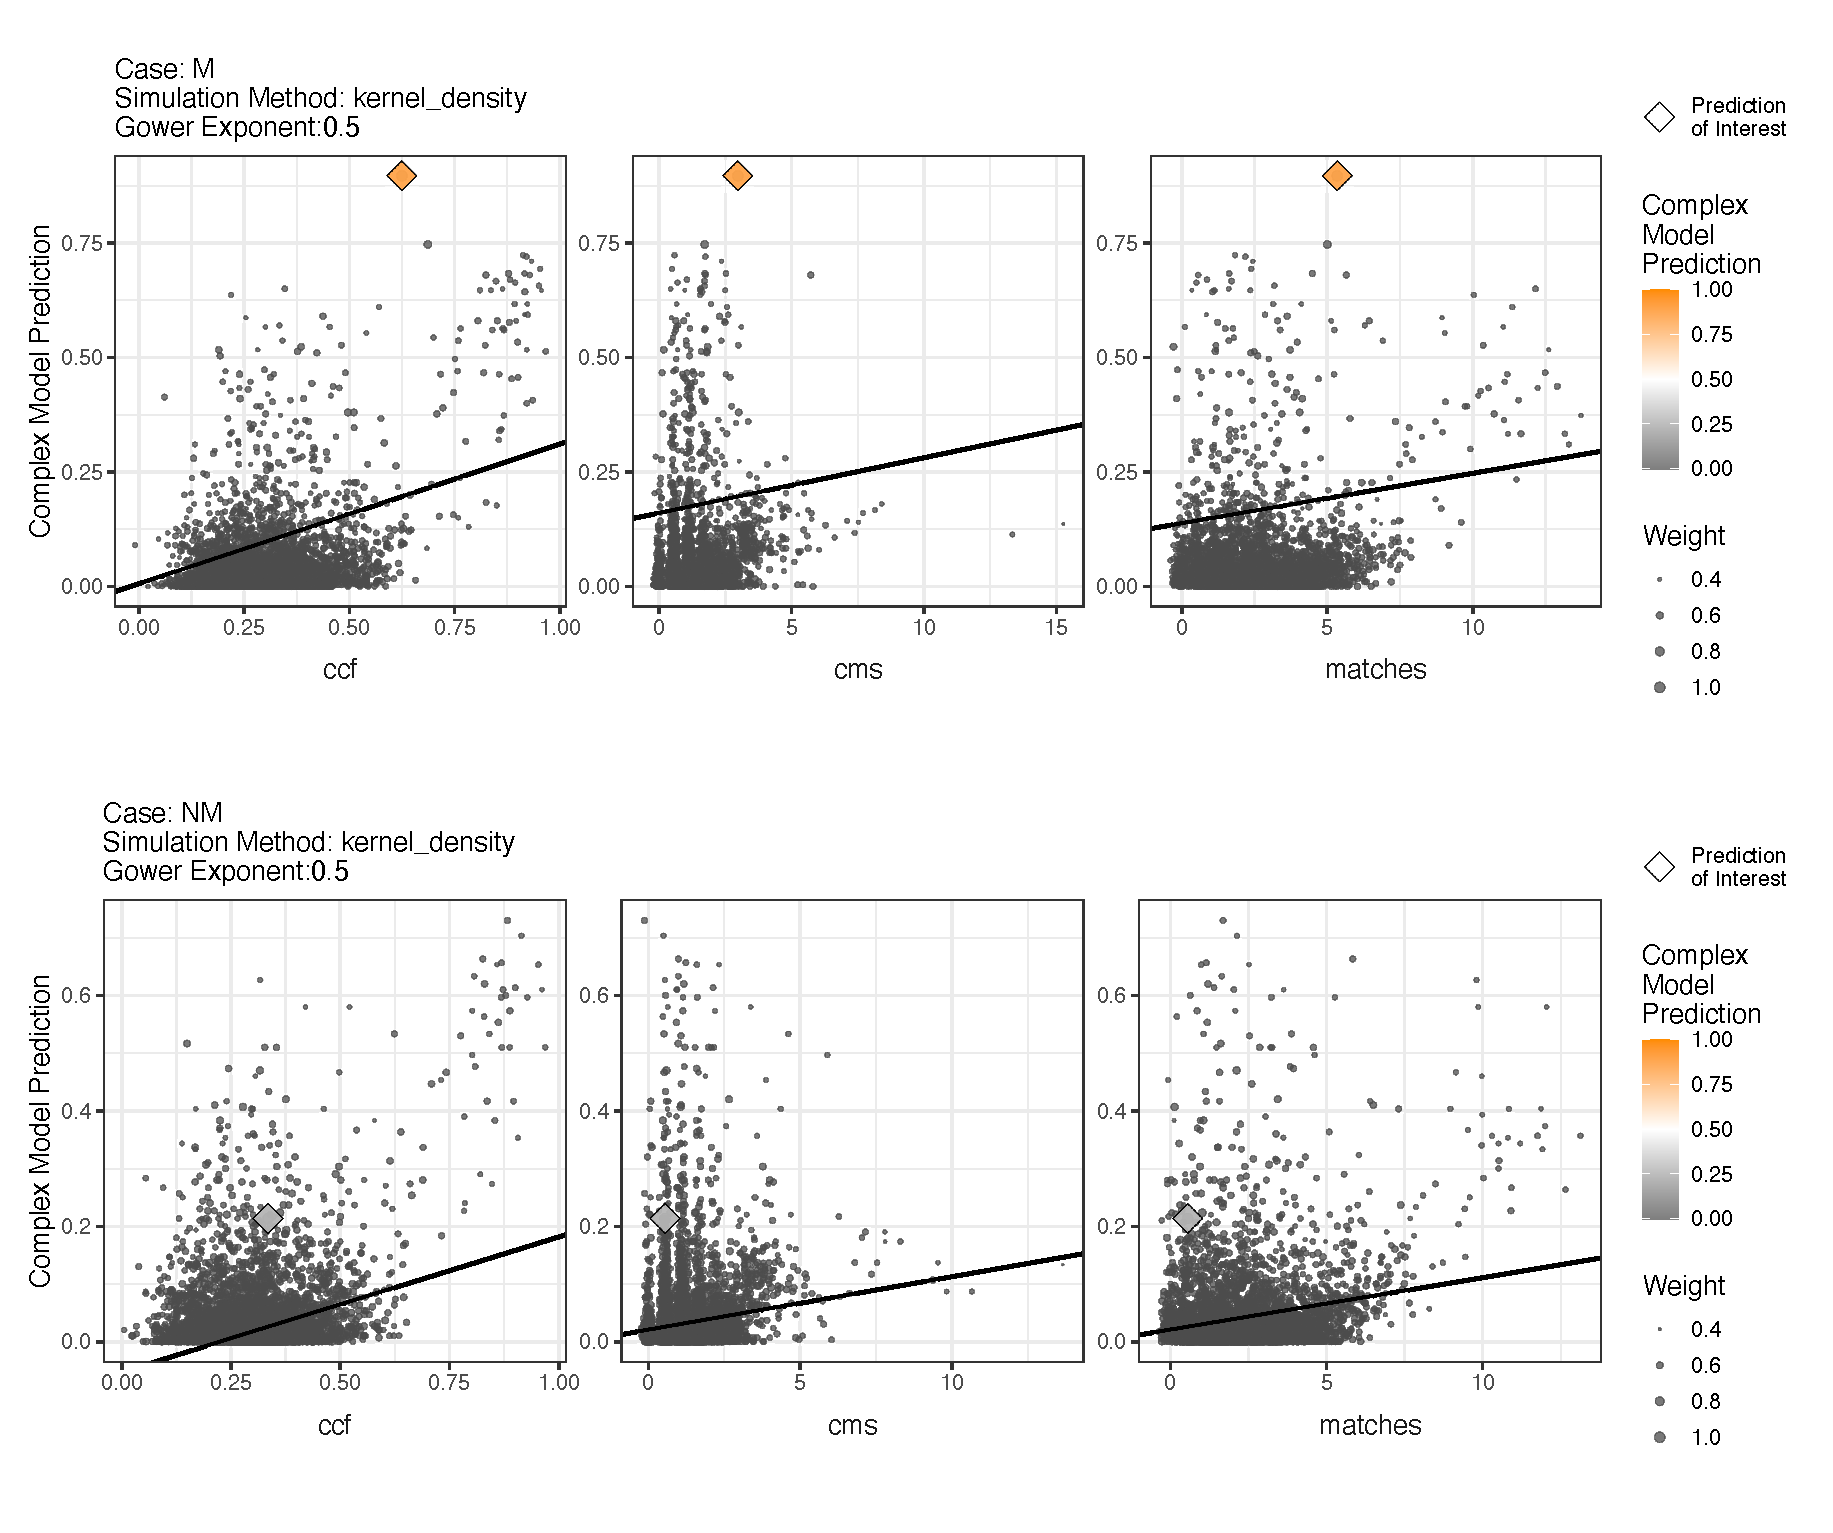
\includegraphics[width=6.5in]{figure-B2-1}
%DIFDELCMD <

%DIFDELCMD < }
%DIFDELCMD <

%DIFDELCMD < \end{knitrout}
%DIFDELCMD < %%%
%DIFDELCMD < \caption{%
{%DIFAUXCMD
\DIFdelFL{Explanation scatterplots for LIME explanations using kernel density simulation for the cases M and NM of the bullet comparison test data.}}
%DIFAUXCMD
%DIFDELCMD < \label{fig:figure-B2}
%DIFDELCMD < \end{figure*}
%DIFDELCMD <

%DIFDELCMD < %%%
\section{\DIFdel{Explainer Model Residual Plot}} %DIFAUXCMD
\addtocounter{section}{-1}%DIFAUXCMD
%DIFDELCMD < \label{residual-plot}
%DIFDELCMD <

%DIFDELCMD < %%%
\DIFdelend In order to assess the claim of linearity for the \data \ prediction of interest discussed in Section \ref{exp-scatter}, we use one of the most basic diagnostics in a statistician's tool box and draw a residual plot for the explainer model. This is shown in \DIFdelbegin \DIFdel{Figure \ref{fig:figure-C3} }\DIFdelend \DIFaddbegin \autoref{fig:figure-B1} \DIFaddend with the explainer model residuals on the y-axis and explainer model predictions on the x-axis. The points along the x-axis have been jittered to ease the effect of the over-plotted points\DIFdelbegin \DIFdel{in the visualization}\DIFdelend . There is a clear increasing trend in the residuals as the explainer model predictions increase\DIFdelbegin \DIFdel{. This is a clear }\DIFdelend \DIFaddbegin \DIFadd{, which indicates a }\DIFaddend violation of the \DIFdelbegin \DIFdel{linearity assumption with the ridge regression model.
}%DIFDELCMD <

%DIFDELCMD < \begin{figure}[!thp]
%DIFDELCMD < \begin{knitrout}
%DIFDELCMD < \definecolor{shadecolor}{rgb}{0.969, 0.969, 0.969}\color{fgcolor}
%DIFDELCMD <

%DIFDELCMD < {\centering 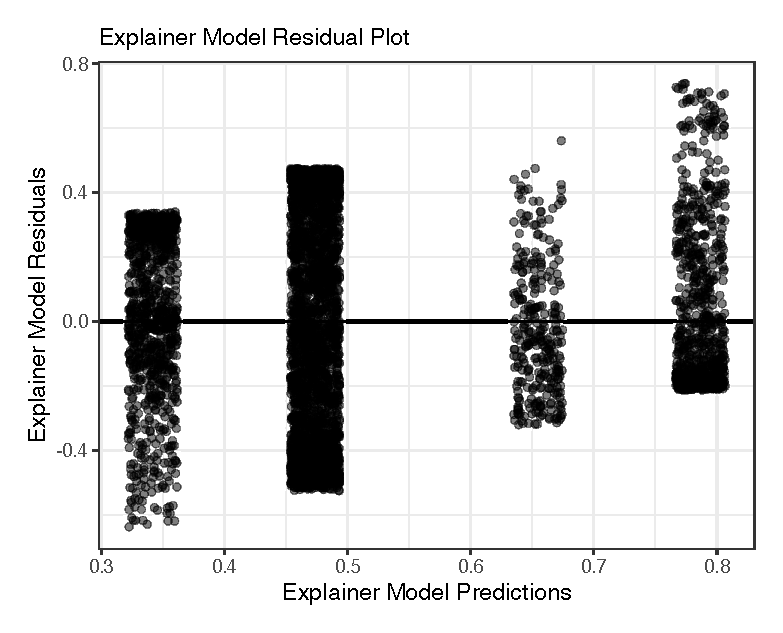
\includegraphics[width=3.125in]{figure-C3-1}
%DIFDELCMD <

%DIFDELCMD < }
%DIFDELCMD <

%DIFDELCMD < \end{knitrout}
%DIFDELCMD < %%%
%DIFDELCMD < \caption{%
{%DIFAUXCMD
\DIFdelFL{Residual plot of the explainer model associated with \data \ prediction of interest from Section \ref{exp-scatter}. The residuals are plotted against the predicted values. The points are jittered in the x-direction to alleviate the over-plotting of points. There is an upward trend in the residuals as the explainer model predictions increase, which suggests a violation of the linearity assumption.}}
%DIFAUXCMD
%DIFDELCMD < \label{fig:figure-C3}
%DIFDELCMD < \end{figure}
%DIFDELCMD < %%%
\DIFdelend \DIFaddbegin \DIFadd{ridge regression linearity assumption.
}\DIFaddend

\section{Details on Assessment Metrics} \label{metric-details}

Suppose $f$ is a complex model, and let $\textbf{X}$ be a matrix of observed data with $K$ features and $E$ observations where $x_e$ is an observed feature vector for observation $e$. Let $f(x_e)$ be the complex model prediction for observation $e$. It is of interest to explain the predictions made by $f$ applied to $X$ using LIME.

For $x_e$ and a set of tuning parameter values $t$, let $\textbf{X}_{e,t}'$ be the LIME simulated dataset with $K$ features and $S$ rows such that $x'_{e,t,s}$ is the feature vector for simulated data point $s$ corresponding to explanation $e$ and tuning parameter values $t$. Let $\textbf{Z}'_{e,t}$ be the matrix of simulated data transformed to bin indicator variables (for bin based simulation methods) or standardization (for density based simulation methods) with $K$ features and $S$ observations such that $z'_{e,t,s}$ is the interpretability transformed feature vector for explanation $e$, tuning parameter values $t$, and simulated data point $s$. Note that $z_{e,t}$ will represent the transformed version of $x_e$.

Next, let $\omega_t$ represent a proximity distance metric corresponding to tuning parameter values $t$. Then $\omega_t\left(x_e, x'_{e,t,s}\right)$ is the weight assigned to $x'_{e,t,s}$, which is the proximity between $x_e$ and $x'_{e,t,s}$. Allow $g_{e,t}$ to be the explainer model for an explanation $e$ and tuning parameter values $t$. Thus, $g_{e,t}\left(z'_{e,s,t}\right)$ is the explainer model prediction for the interpretability transformed simulated data point $s$.

For a set of $E$ explanations and a set of tuning parameter values $t$, we define the assessment metrics as follows:\\
\\
\emph{Average $R^2$} is denoted as $R^2_{\mbox{ave}}$ and computed as

  $$R^2_{\mbox{ave}} = \frac{1}{E}\sum_{e=1}^E R_{e,t}^2$$

\noindent where $R_{e,t}^2$ is the $R^2$ value for $g_{e,t}$.\\
\\
\emph{Average fidelity} is denoted by $\mathcal{L}_{\mbox{ave}}$ and computed as

\begin{eqnarray*} \mathcal{L}_{\mbox{ave}} & = & \frac{1}{E}\sum_{e=1}^E\mathcal{L}(f, \ g_{e,t}, \ \pi_{t}) \\ & = & \frac{1}{E}\sum_{e=1}^E\sum_{s=1}^{S}\omega_{t}\left(x_e, x'_{e,t,s}\right)\left(f\left(x'_{e,t,s}\right)-g_{e,t}\left(z_{e,t,s}'\right)\right)^2. \end{eqnarray*}

\noindent where $\mathcal{L}$ is the fidelity metric originally defined in \citet{ribeiro:2016}.\\
\\
\emph{Mean squared explanation error} is denoted by MSEE and computed as

$$MSEE=\frac{1}{E}\sum_{e=1}^E\left(f\left(x_e\right)-g_{e,t}\left(z_{e,t}\right)\right)^2.$$

\end{document}
